% Settings for the default beamer theme
\documentclass[english, aspectratio=169]{beamer}
\usepackage[T1]{fontenc}
\usepackage[utf8]{inputenc}
\usepackage{tabularx}
\usepackage{babel}
\usepackage[ruled,vlined]{algorithm2e}
\SetAlgorithmName{Algoritmus}{algoritmus}{List of Algorithms}
\setcounter{secnumdepth}{3}
\setcounter{tocdepth}{3}

\makeatletter

\newcommand\makebeamertitle{\frame{\maketitle}}

% (ERT) argument for the TOC
\AtBeginDocument{%
  \let\origtableofcontents=\tableofcontents
  \def\tableofcontents{\@ifnextchar[{\origtableofcontents}{\gobbletableofcontents}}
  \def\gobbletableofcontents#1{\origtableofcontents}
}

% Theme settings
\usetheme{Frankfurt}
\usecolortheme{default}
\usefonttheme[onlymath]{serif}

% Template settings
\setbeamertemplate{navigation symbols}{}
\setbeamertemplate{blocks}[rounded][shadow=false]
\setbeamertemplate{title page}[default][colsep=-4bp, rounded=true, shadow=false]
\makeatother

% Define a custom darker red color
\definecolor{DarkerRed}{RGB}{139,0,0} % Adjust the RGB values as needed

% Use the newly defined color in Beamer theme elements
\setbeamercolor{structure}{fg=DarkerRed} % Changes basic structural elements to Darker Red
\setbeamercolor{title in head/foot}{bg=DarkerRed} % Changes the title in header/footer to Darker Red


\begin{document}

% Title page
\section{Bevezetés}
\title[]{Üzleti Elemzések Módszertana}
\subtitle{8. Előadás: Generatív modellezés}
\author[Kuknyó Dániel]{Kuknyó Dániel\\Budapesti Gazdasági Egyetem}
\date{2023/24\\2.félév}
\makebeamertitle

% Table of contents slide
\begin{frame}
\tableofcontents{}
\end{frame}

% Table of contents of the current section
\begin{frame}
\tableofcontents[currentsection]
\end{frame}

\begin{frame}{Diszkriminatív modellezés}
\begin{columns}
\begin{column}{.5\textwidth}
Diszkriminatív modellezés esetén a modellezés eljárása:
\begin{enumerate}
	\item Tanító adatok gyűjtése
	\item Modell tanítása a tanító adatokon
	\item Nem látott mintaegyedeken predikció elvégzése
\end{enumerate}
\end{column}
\begin{column}{.5\textwidth}
\begin{center}
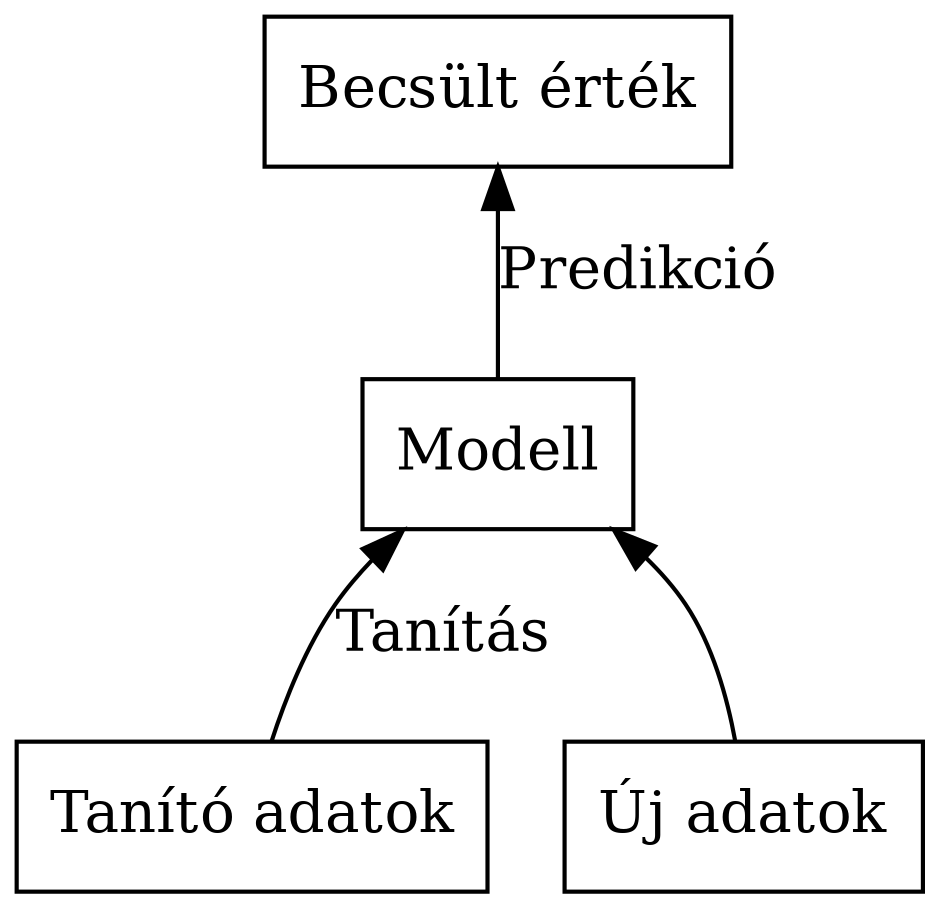
\includegraphics[width=6cm, height=6cm, keepaspectratio]{graphs/generative_2.png}
\end{center}
\end{column}
\end{columns}
\end{frame}

\begin{frame}{Generatív modellezés}
\begin{columns}
\begin{column}{.5\textwidth}
Generatív modellezés esetén a folyamat a következőképpen módosul:
\begin{enumerate}
	\item Tanító adatok gyűjtése
	\item Modell tanítása a tanító adatokon
	\item Zaj beengedése a rendszerbe
	\item Új mintaegyed létrehozása
\end{enumerate}
\end{column}
\begin{column}{.5\textwidth}
\begin{center}
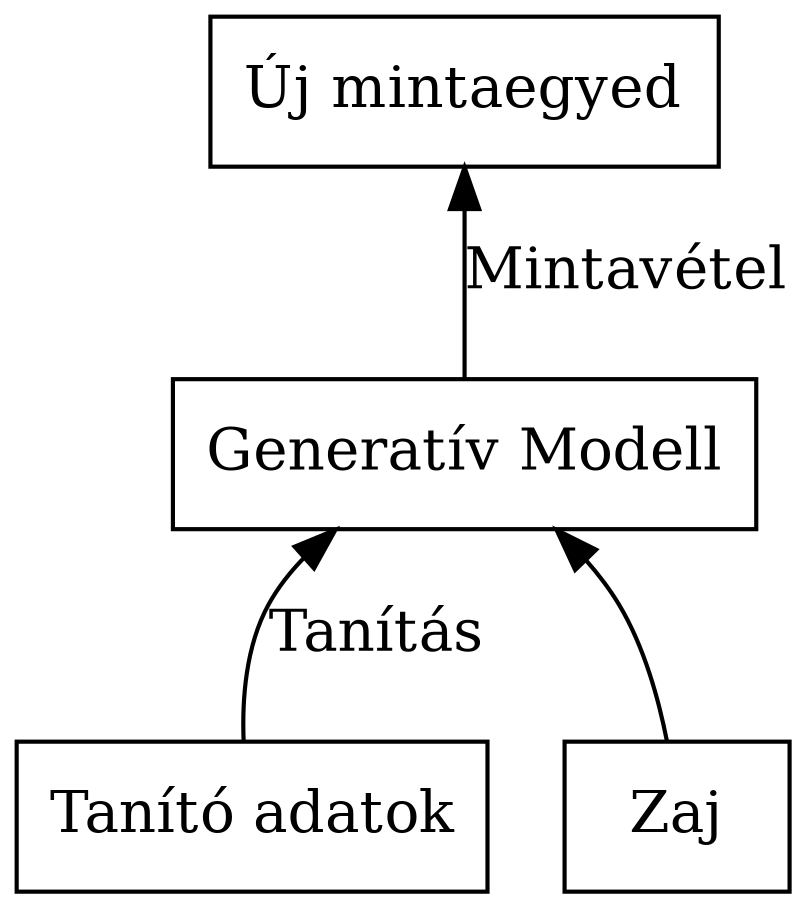
\includegraphics[width=6cm, height=6cm, keepaspectratio]{graphs/generative_3.png}
\end{center}
\end{column}
\end{columns}
\end{frame}

\begin{frame}{Diszkriminatív modellezés}
\begin{columns}
\begin{column}{.5\textwidth}
\begin{block}{Diszkriminatív modell}
A tanítás, hogy megkülönböztesse a különböző adatkategóriákat. Ezt használja fel arra, hogy megbecsülje az adatpontok osztályba tartozását.
\end{block}
\end{column}
\begin{column}{.5\textwidth}
\begin{center}
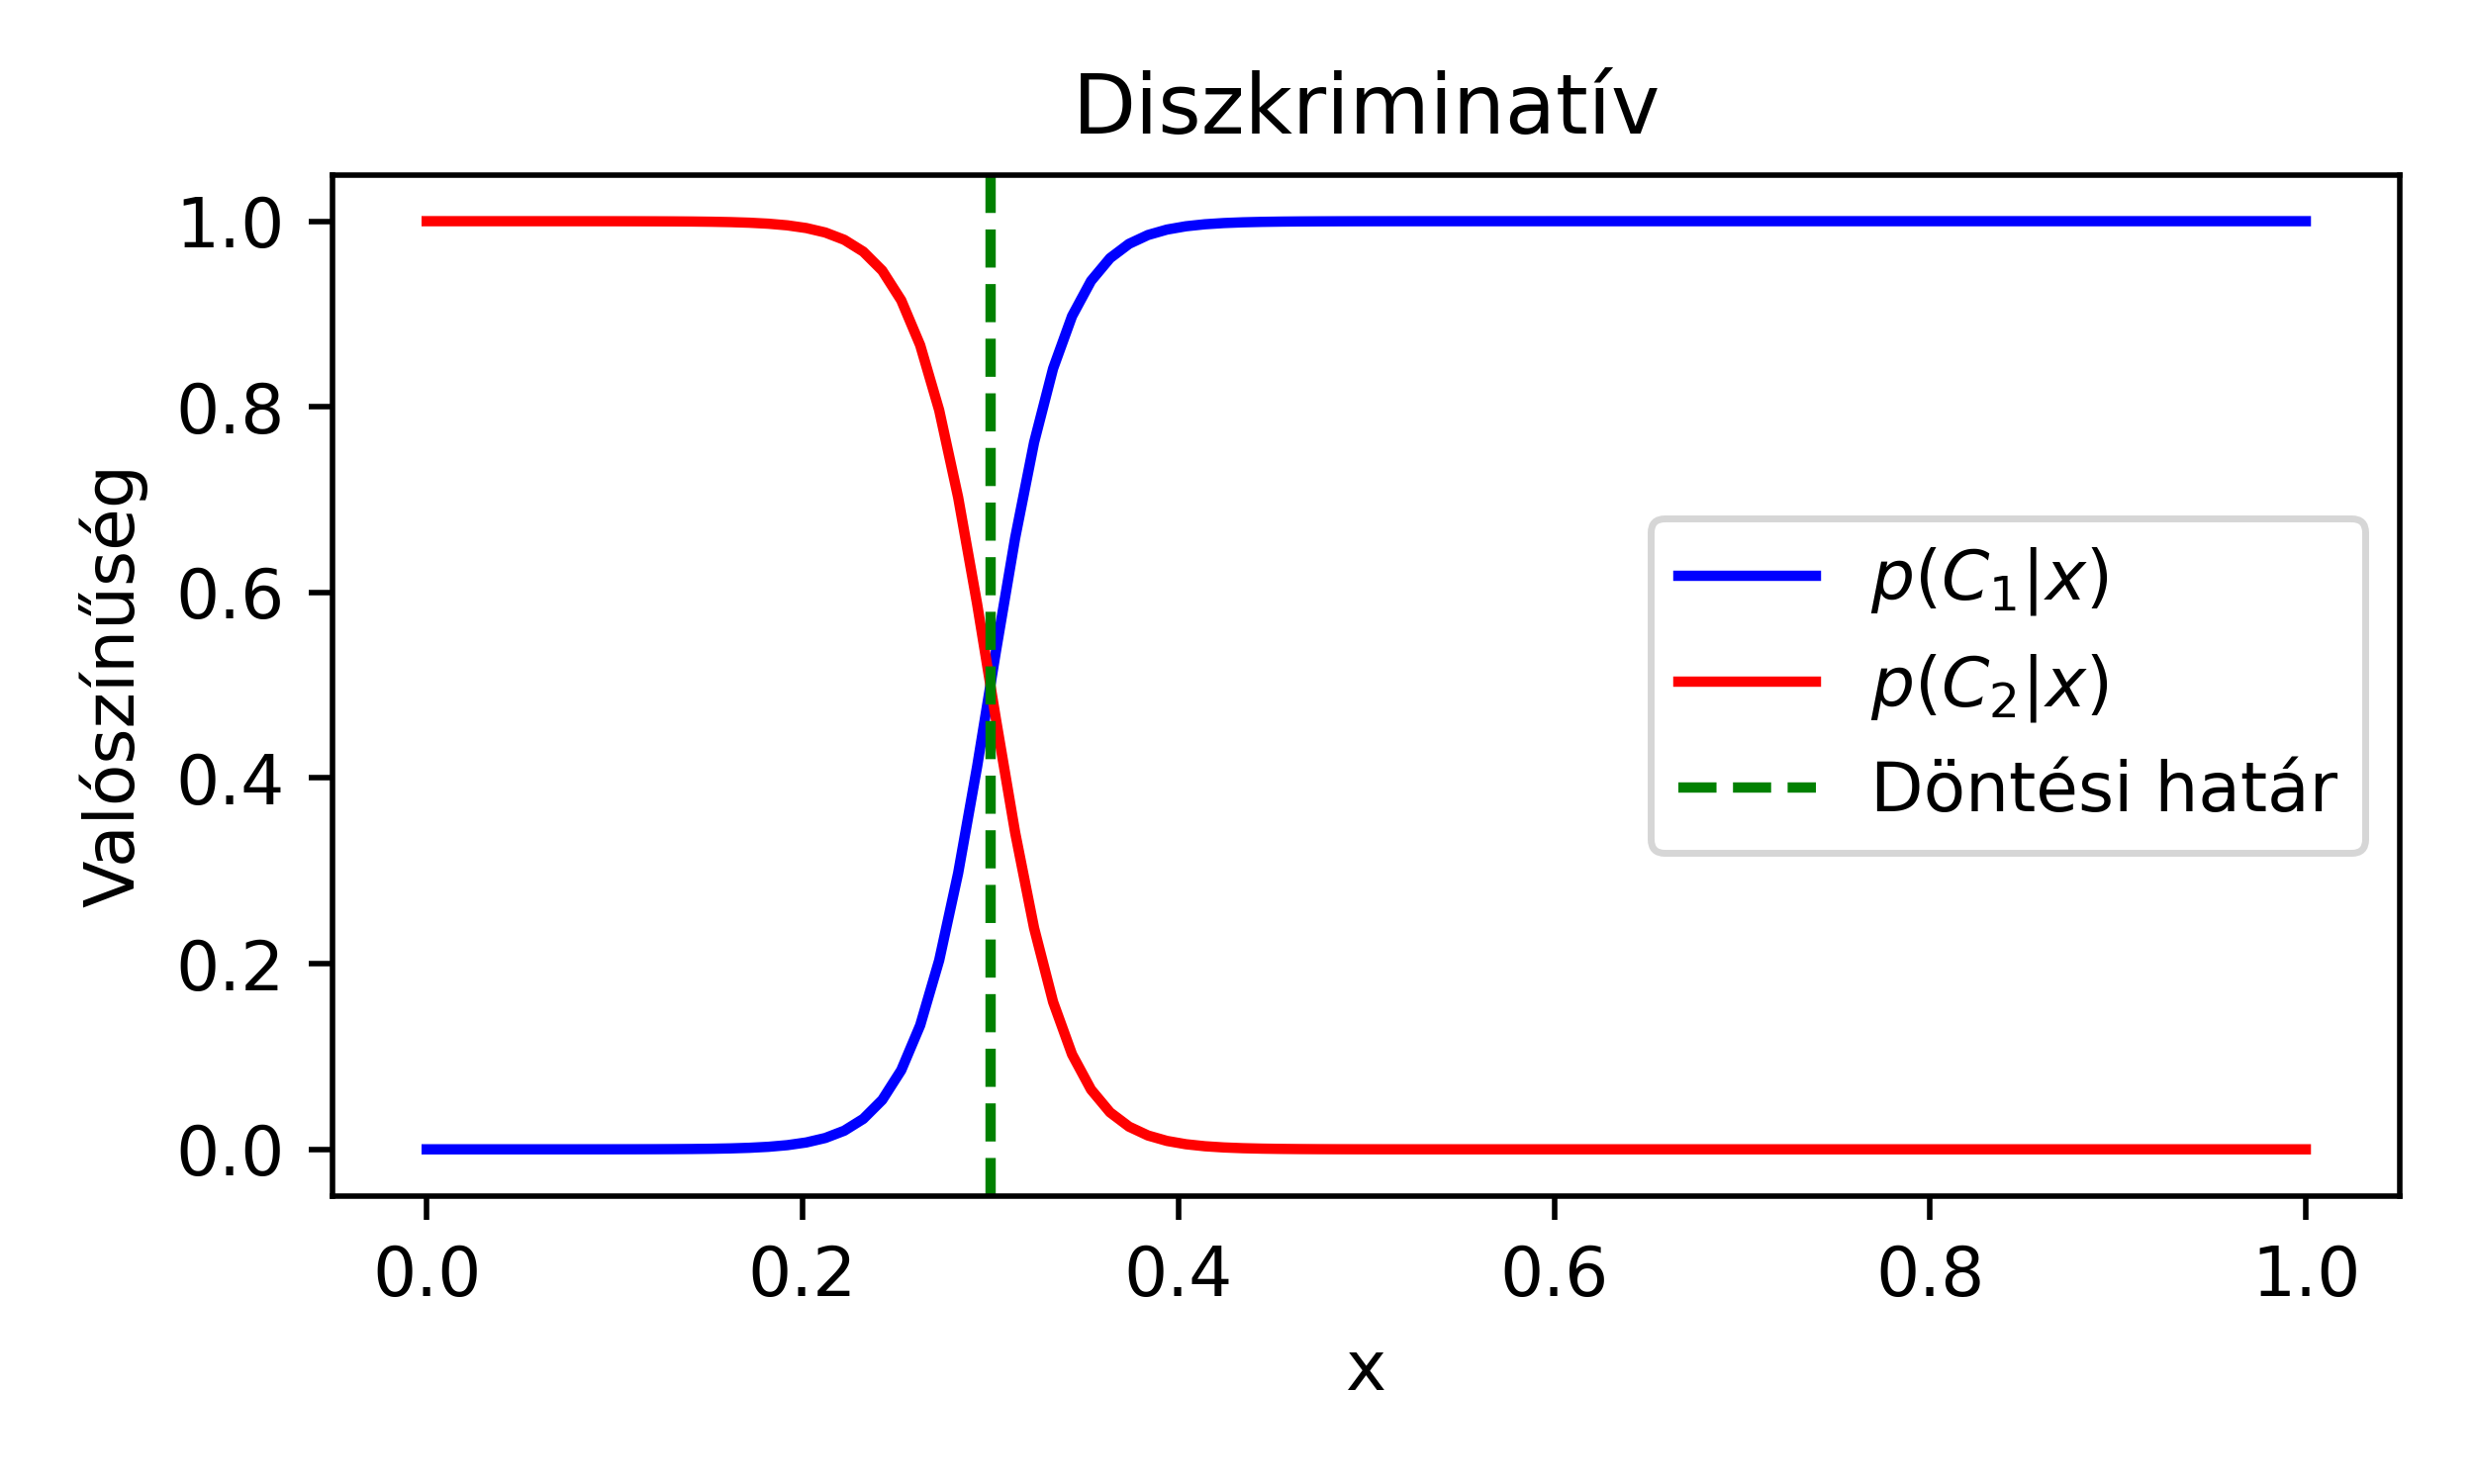
\includegraphics[width=7cm, height=7cm, keepaspectratio]{images/generative_1.png}
\end{center}
\end{column}
\end{columns}
\end{frame}

\begin{frame}{Generatív modellezés}
\begin{columns}
\begin{column}{.5\textwidth}
\begin{block}{Generatív modell}
A célja, hogy megtanulja az adatok eloszlását. Megtanulja, hogyan generálódnak az adatok, és ezt felhasználva képesek új adatokat generálni.
\end{block}
\end{column}
\begin{column}{.5\textwidth}
\begin{center}
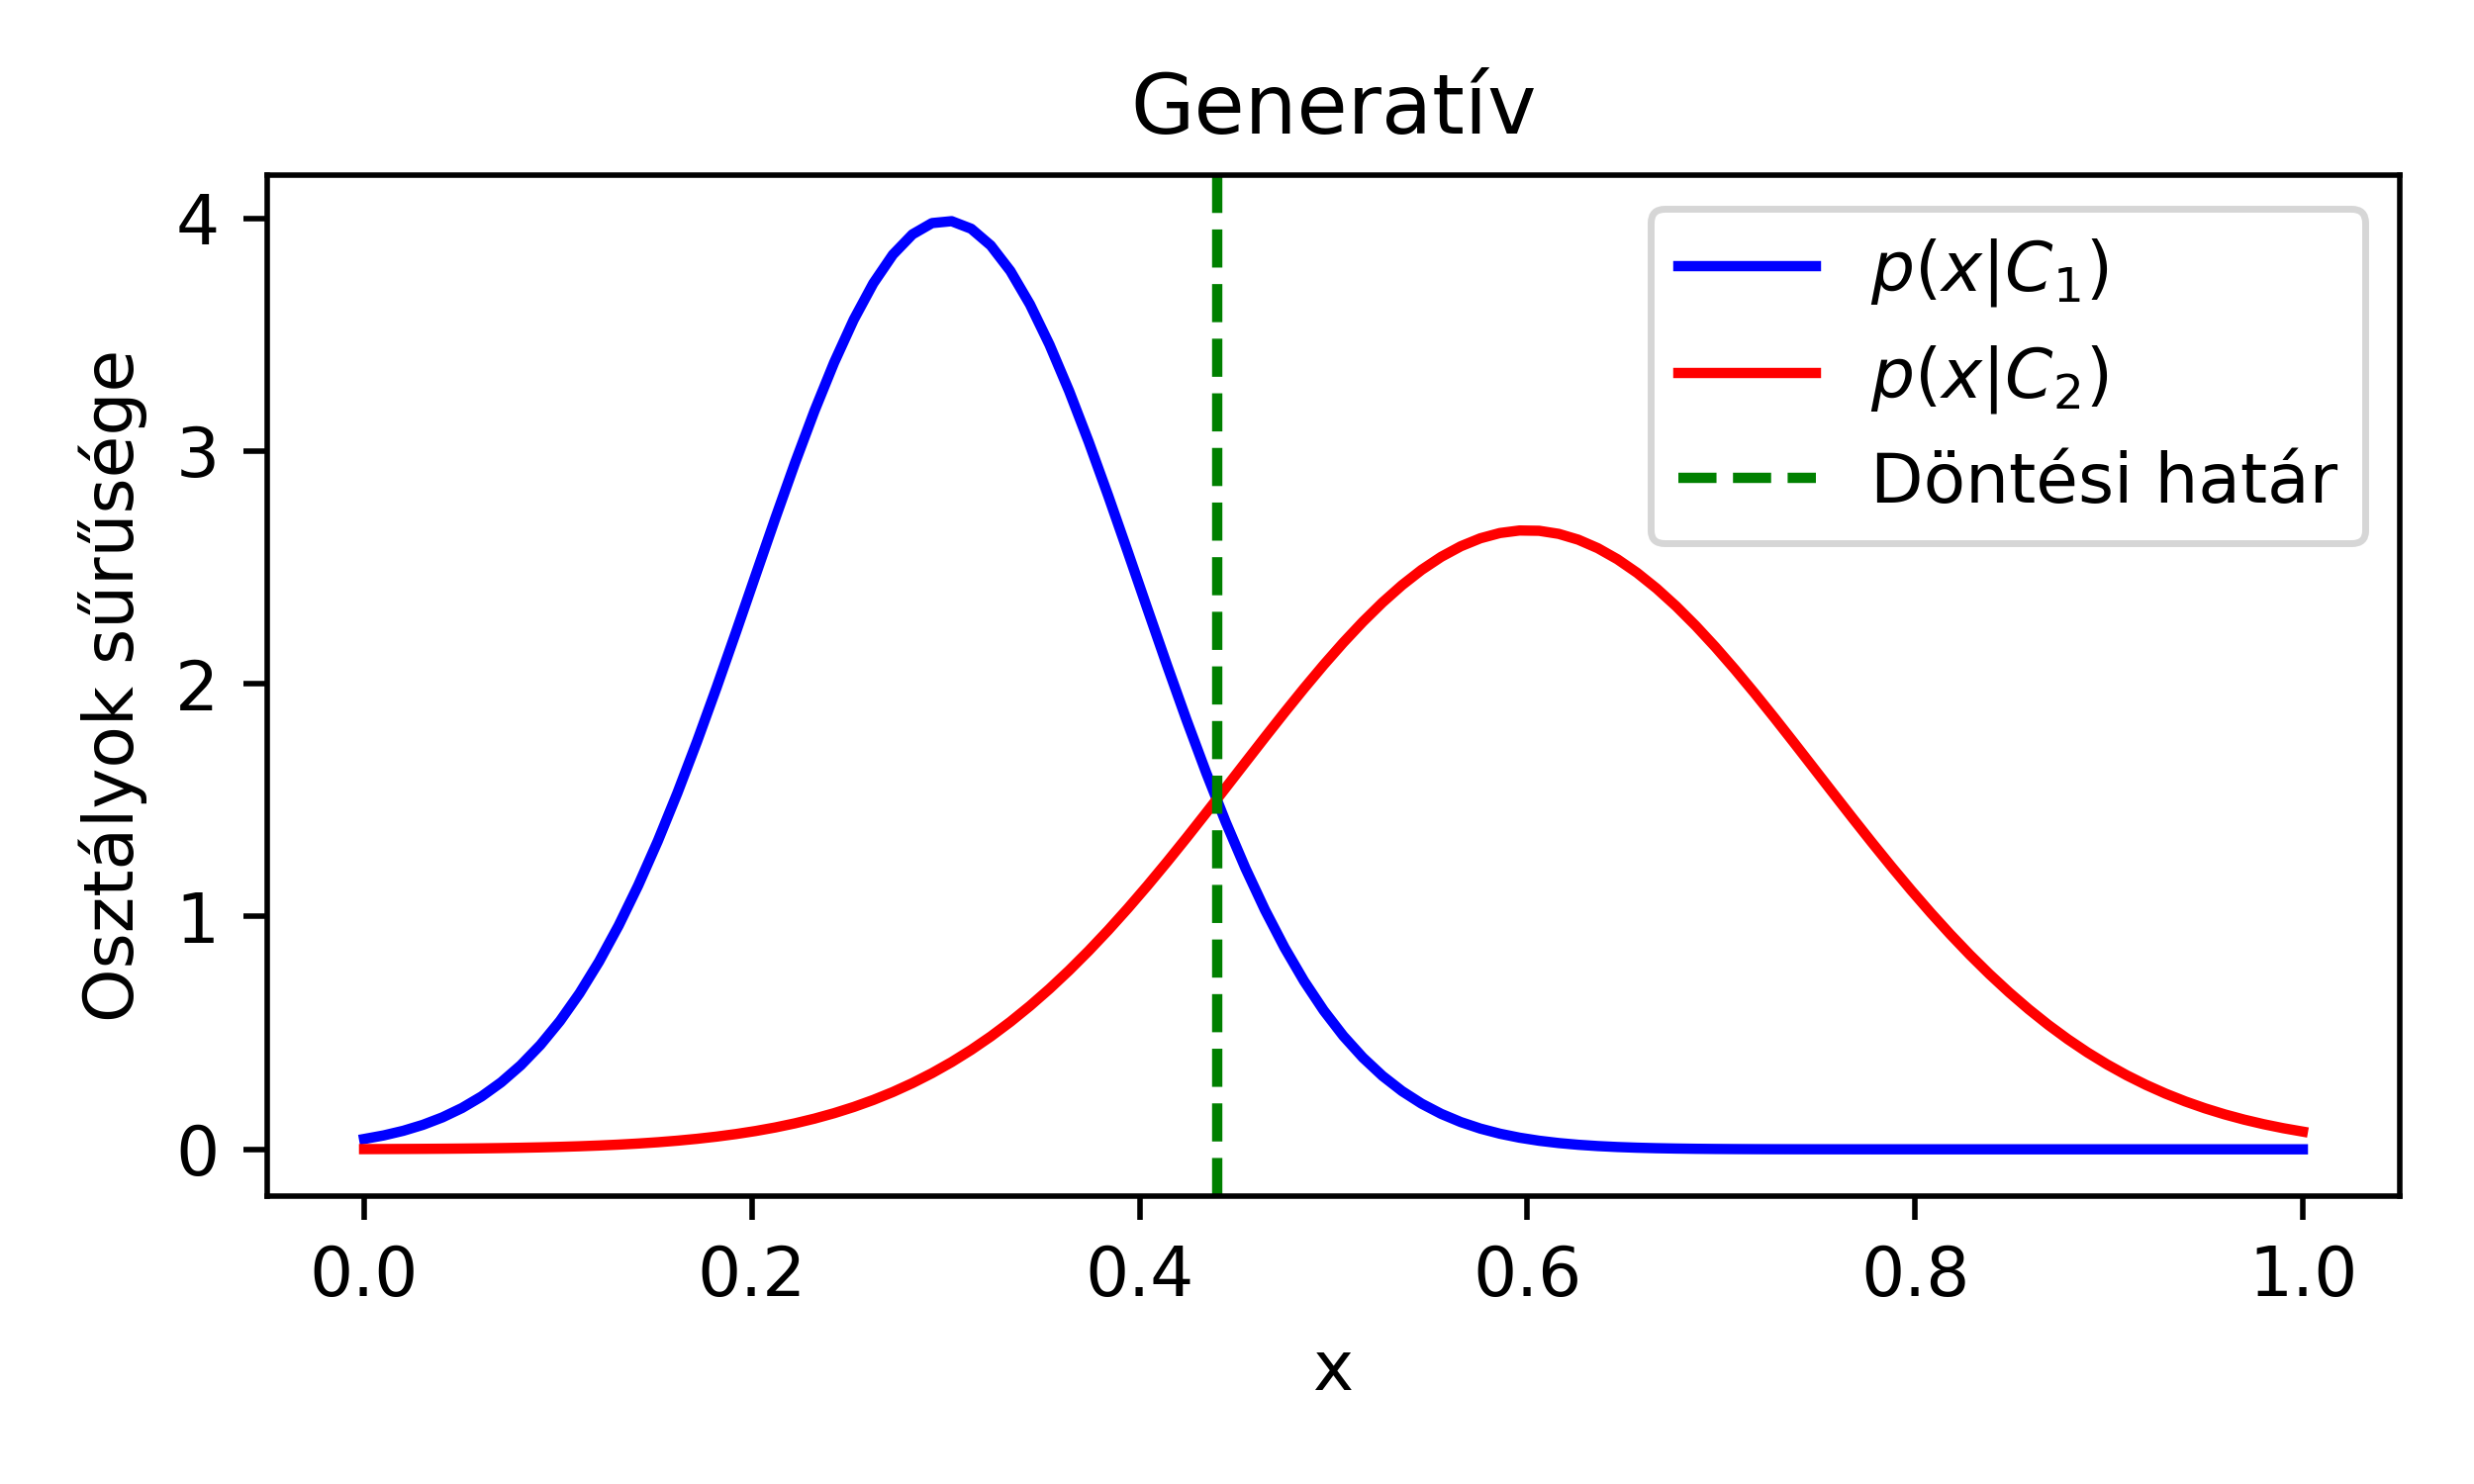
\includegraphics[width=7cm, height=7cm, keepaspectratio]{images/generative_2.png}
\end{center}
\end{column}
\end{columns}
\end{frame}

\begin{frame}{Feltételes valószínűségek}
\begin{columns}
\begin{column}{.5\textwidth}
Valamely $A$ esemény feltételes valószínűsége azt jelenti, mekkora az esély $A$ esemény bekövetkezésére feltéve, hogy $B$ esemény már megtörtént. Ennek jelölése:
\begin{block}{}
\[
P\left( A \vert B \right) = \frac{P\left( A \cap B \right)}{P\left( B \right)}
\]
\end{block}
Ennek megfelelően például az a valószínűség, hogy egy rendelés csalóktól érkezik feltéve, hogy kupont használtak: 
\begin{block}{}
\vspace{-.4cm}
\[
P\left( \text{Csaló} \vert	\text{Kupon} \right) = \frac{P\left( \text{Csaló} \cap \text{Kupon} \right)}{P\left( \text{Kupon} \right)}
\]
\end{block}
\end{column}
\begin{column}{.5\textwidth}
\begin{center}
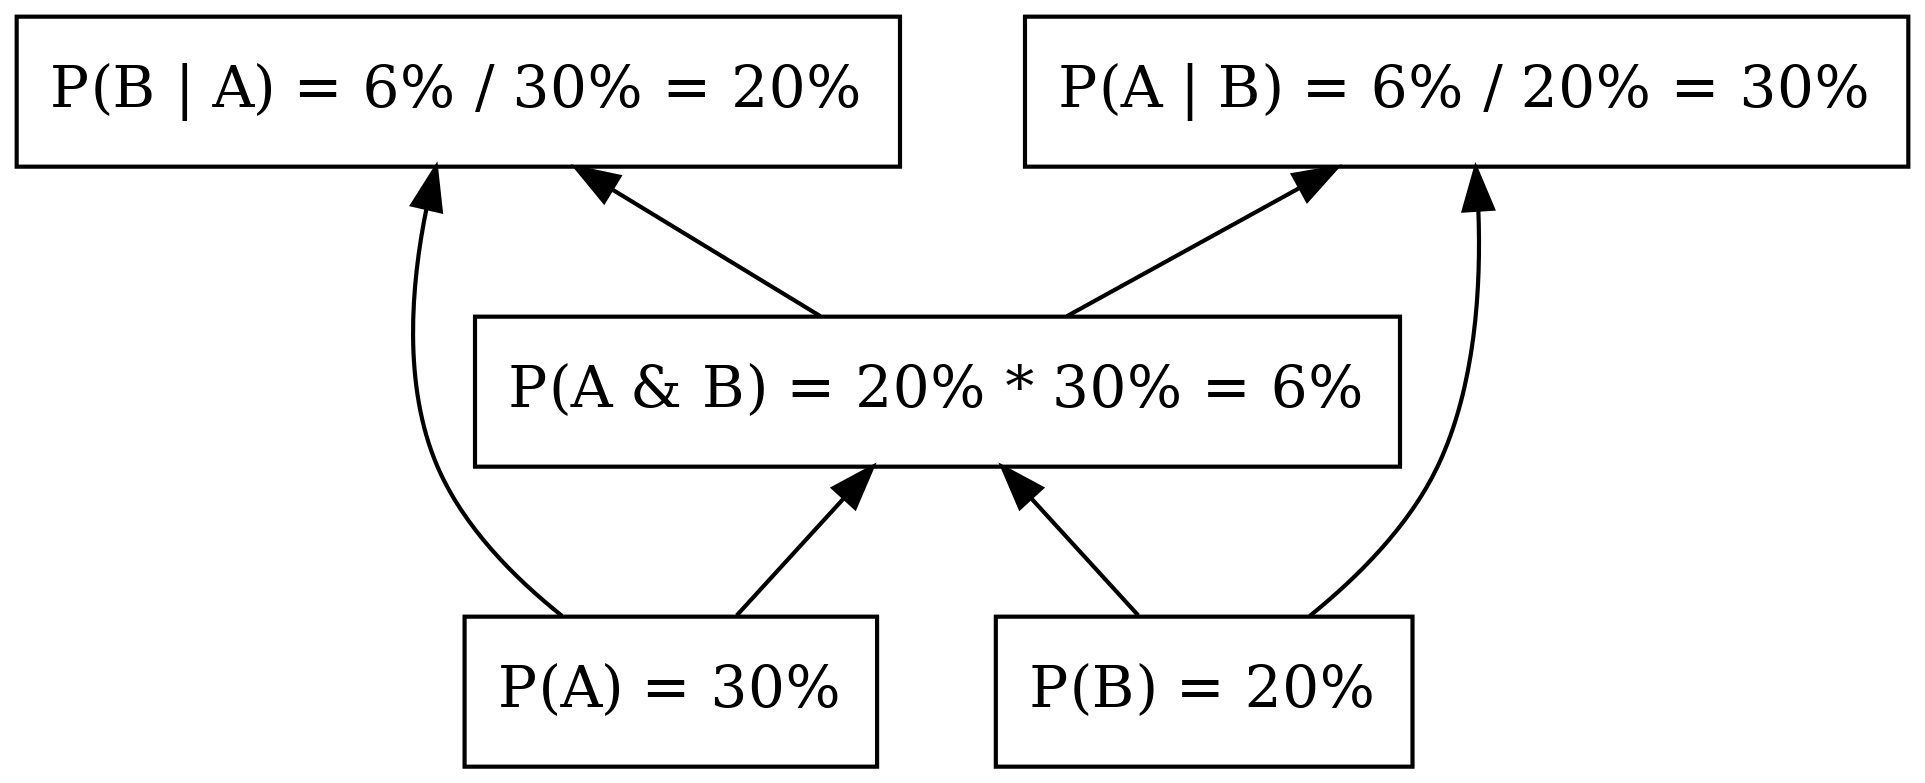
\includegraphics[width=7cm, height=7cm, keepaspectratio]{graphs/generative_1.png}
\end{center}
\end{column}
\end{columns}
\end{frame}

\begin{frame}{Inverz feltételes valószínűségek}
\begin{columns}
\begin{column}{.4\textwidth}
Az inverz feltételes valószínűség kiszámítható a \textbf{Bayes-tételnek megfelelően a feltételes valószínűség és a nem feltételes valószínűségek segítségével}:
\begin{block}{}
\vspace{-.3cm}
\[
P\left( B \vert A \right) = \frac{P\left( A \vert B \right) P\left( B \right)}{P\left( A \right)}
\]
\end{block}
\end{column}
\begin{column}{.6\textwidth}
A probabilisztikus modellek ezt veszik alapul. A probabilisztikus osztályozás célja valamely $\mathcal{L}$ címkehalmaz valószínűségét megbecsülni adott $x$ változóhalmaz alapján:
\begin{block}{}
\[
P\left( \mathcal{L} \vert x \right) = \frac{P\left( x \vert \mathcal{L} \right)P\left( \mathcal{L} \right)}{P\left( x \right)}
\]
\end{block}
Ebben az esetben az a valószínűség, hogy egy vásárlás csalóktól érkezik feltéve, hogy kupont használtak:
\begin{block}{}
\vspace{-.3cm}
\[
P\left( \text{Csaló} \vert \text{Kupon} \right) = \frac{P\left( \text{Kupon} \vert \text{Csaló} \right)P\left( \text{Csaló} \right)}{P\left( \text{Kupon} \right)}
\]
\end{block}
\end{column}
\end{columns}
\end{frame}

\section{Naív Bayes}

\begin{frame}
\tableofcontents[currentsection]
\end{frame}

\begin{frame}{Naív Bayes}
\begin{columns}
\begin{column}{.5\textwidth}
Probabilisztikus osztályozók egy családja, amely a Bayes-tételt alkalmazza jellemzőkre úgy, hogy közben erősen függetlennek tekinti a jellemzőket.\par\medskip
A naív Bayes modell naivitása abból a feltételezésből ered, hogy egy jellemző jelenléte független bármely másik jellemző jelenlététől, ha adott egy osztály változó. Ez jelentősen csökkenti az algoritmus számítási igényét. 
\end{column}
\begin{column}{.5\textwidth}
\begin{center}
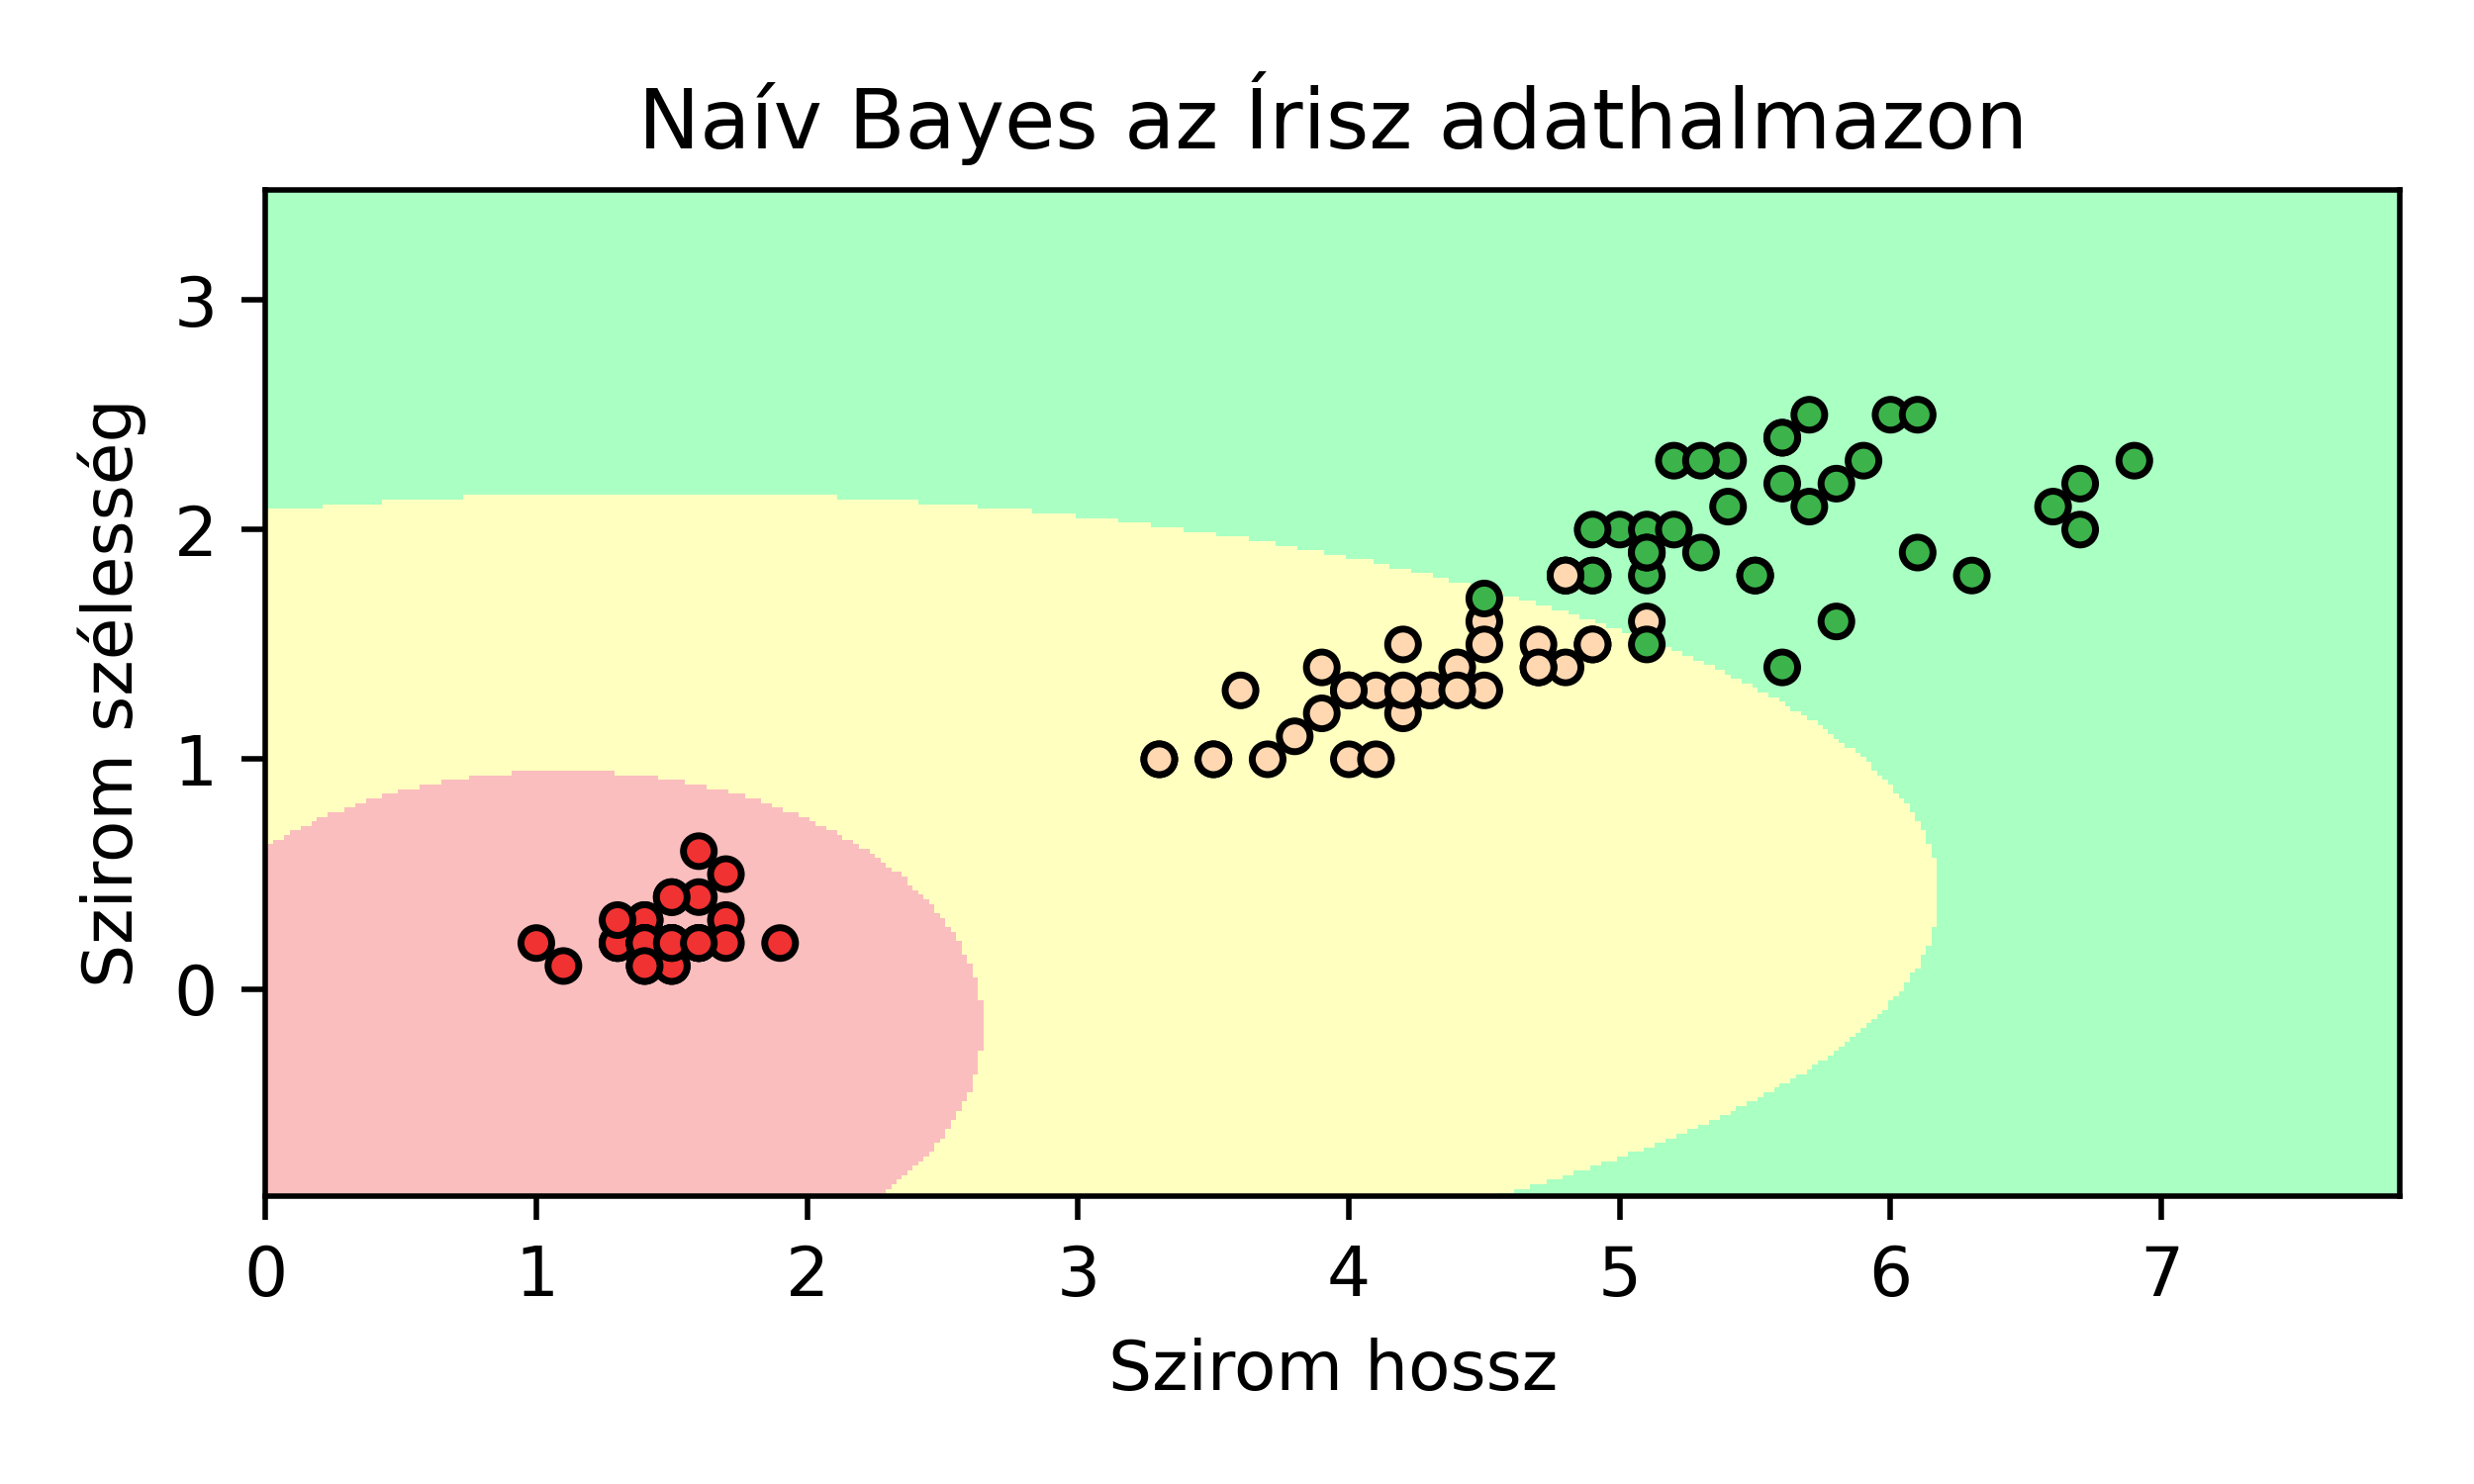
\includegraphics[width=7cm, height=7cm, keepaspectratio]{images/generative_3.png}
\end{center}
\end{column}
\end{columns}
\end{frame}

\begin{frame}{A Gauss-eloszlás}
\begin{columns}
\begin{column}{.6\textwidth}
Egy $X$ véletlen változó Gauss-i eloszlást követ, ha a valószínűség eloszlása a következő függvényt követi:
\begin{block}{Gauss-eloszlás}
\vspace{-.3cm}
\[
f(x \vert \mu, \Sigma) = \frac{1}{\sqrt{(2\pi)^n \vert \Sigma \vert}} e^{\left(-\frac{1}{2}(x - \mu)^T \Sigma^{-1} (x - \mu)\right)}
\]
Ahol:
\begin{itemize}
	\item $\mu$: Az eloszlás várható értéke, vagyis a középre húzás tendenciája
	\item $\Sigma$: A kovarianciamátrix, amely megadja az adatok szóródásának mértékét minden dimenzióban
\end{itemize}
\end{block}
\end{column}
\begin{column}{.4\textwidth}
\begin{center}
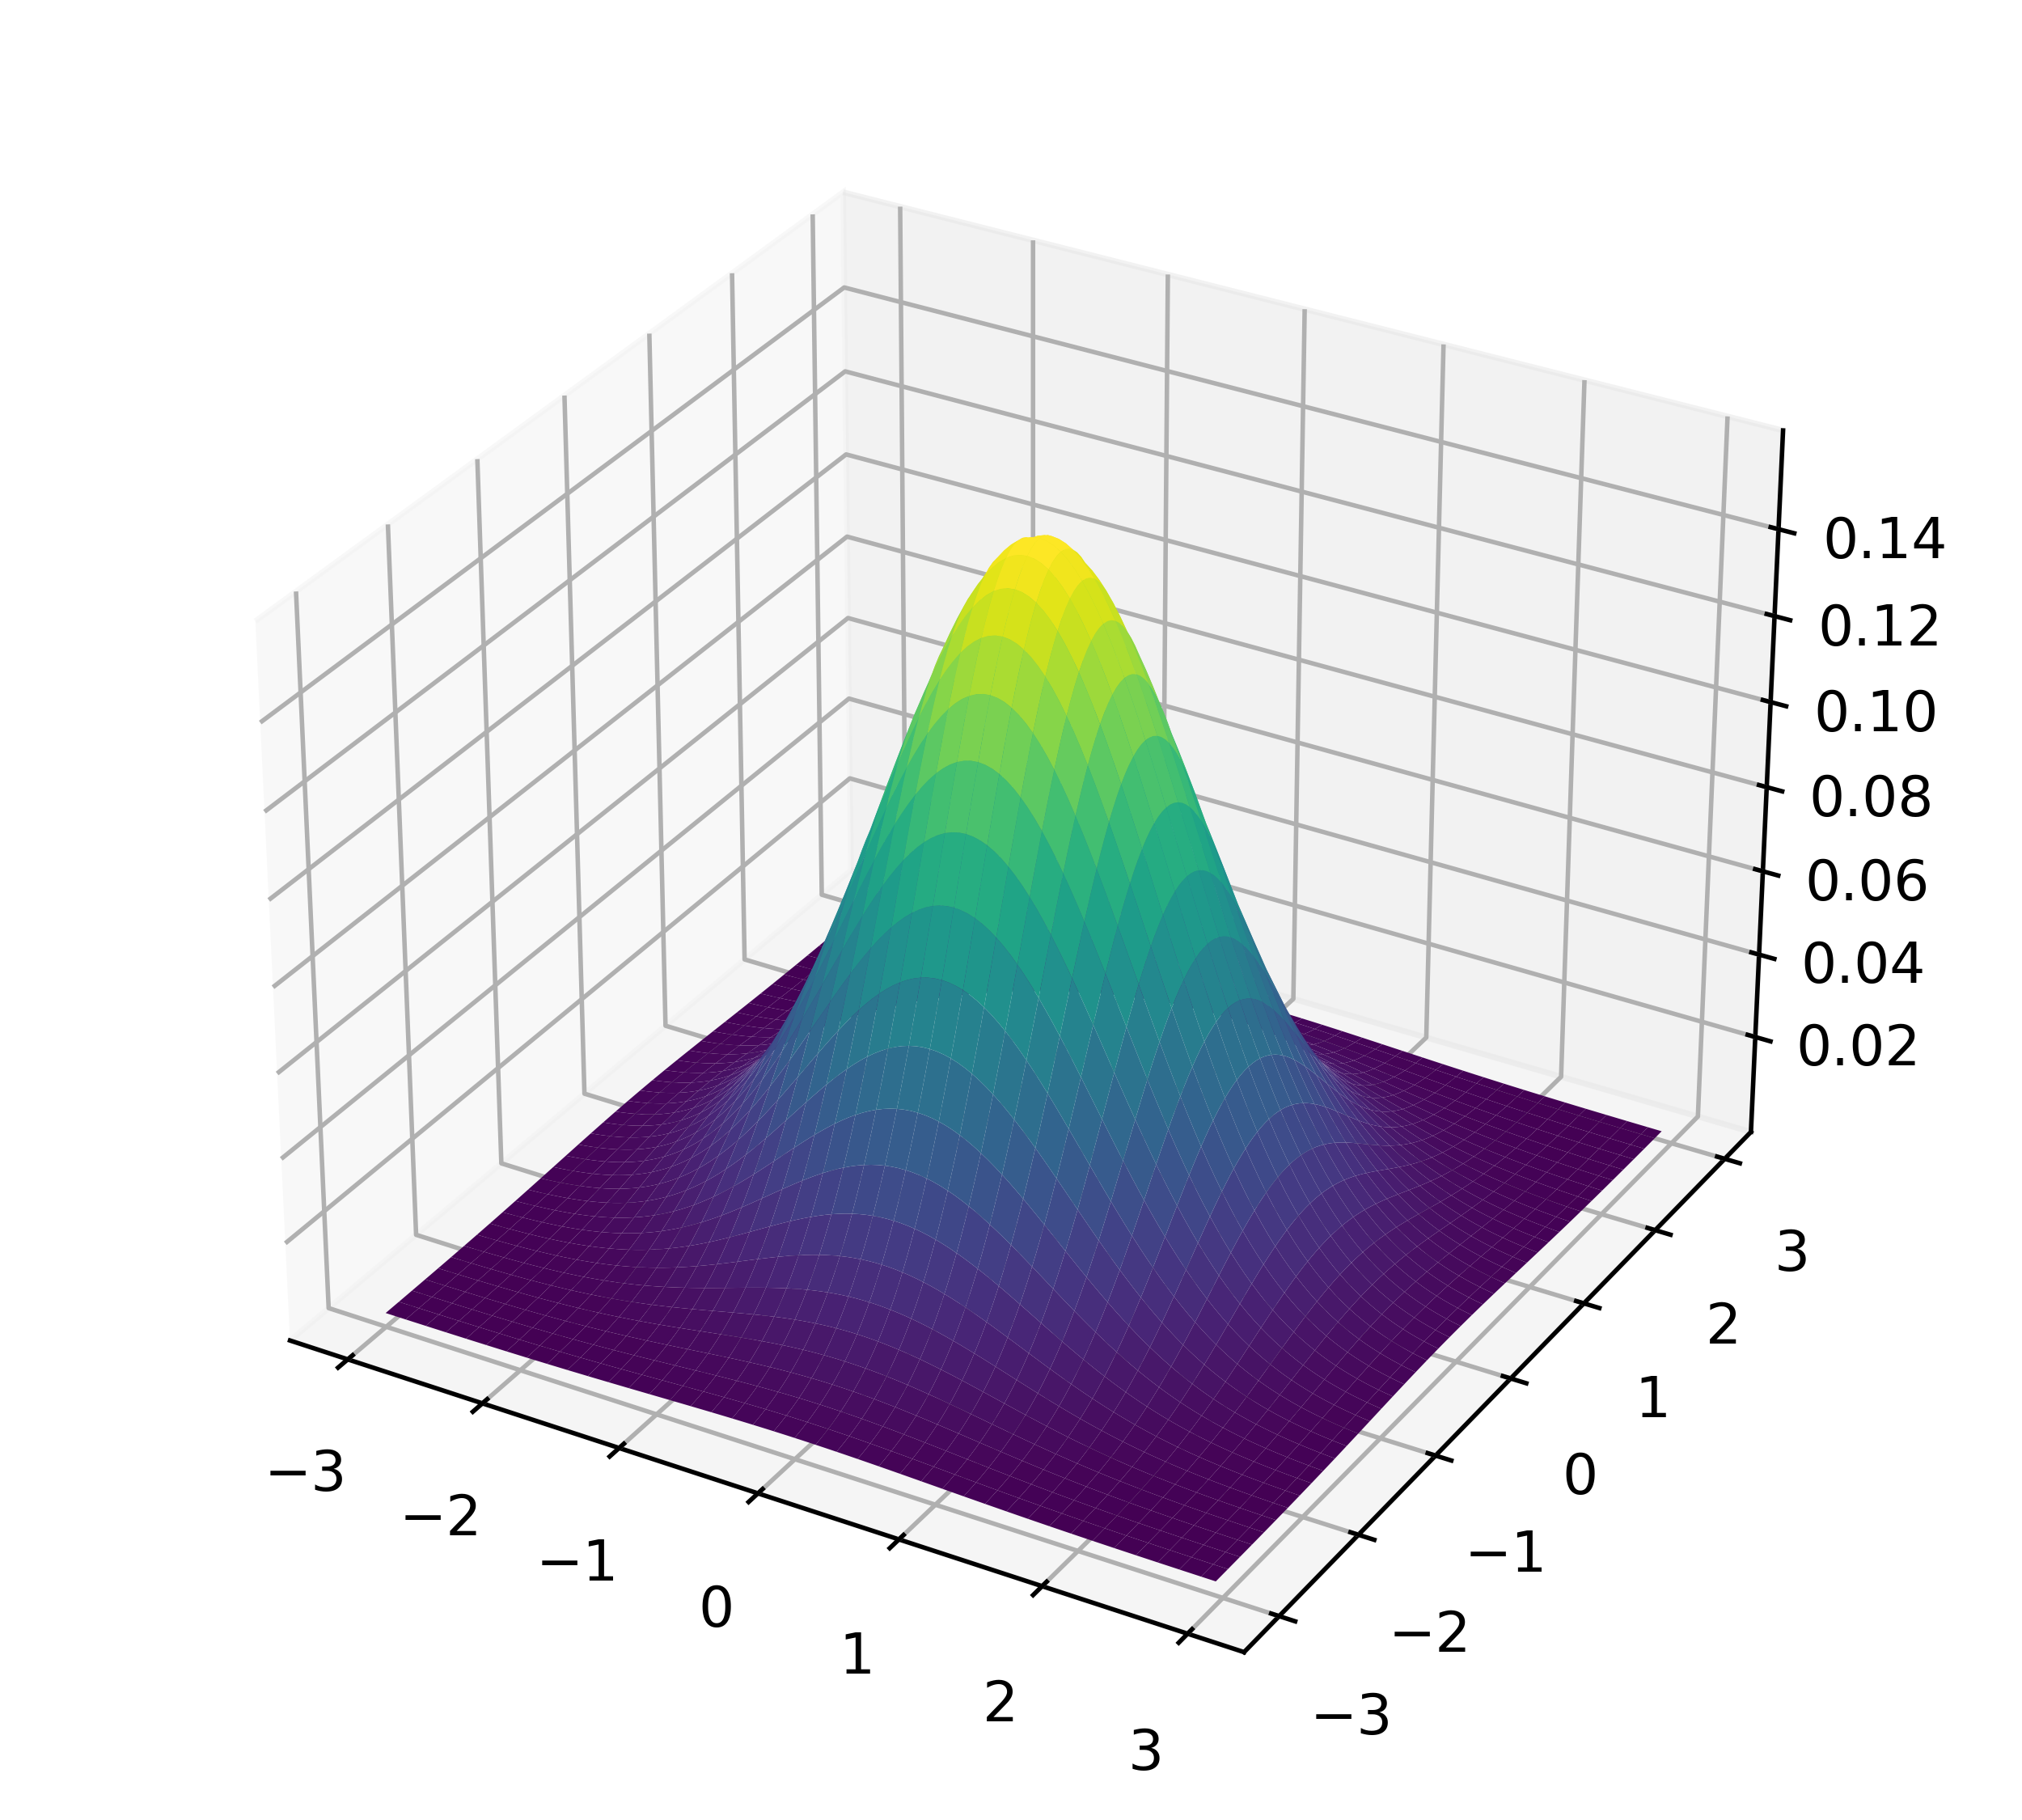
\includegraphics[width=6cm, height=7cm, keepaspectratio]{images/generative_10.png}
\end{center}
\end{column}
\end{columns}
\end{frame}

\begin{frame}{Példák Gauss-eloszlásra}
\begin{columns}
\begin{column}{.3\textwidth}
Az ábrán a következő paraméterekkel definiált többváltozós Gauss-eloszlások láthatók:\par
\only<1>{
\begin{block}{}
\[
\mu = \begin{pmatrix}
0 \\
0
\end{pmatrix}
\]
\[
\Sigma = \begin{pmatrix}
1 & 0 \\
0 & 1
\end{pmatrix}
\]
\end{block}}
\only<2>{
\begin{block}{}
\[
\mu = \begin{pmatrix}
0 \\
0.5
\end{pmatrix}
\]
\[
\Sigma = \begin{pmatrix}
1 & 0 \\
0 & 1
\end{pmatrix}
\]
\end{block}}
\only<3>{
\begin{block}{}
\[
\mu = \begin{pmatrix}
1.5 \\
-0.5
\end{pmatrix}
\]
\[
\Sigma = \begin{pmatrix}
1 & 0 \\
0 & 1
\end{pmatrix}
\]
\end{block}}
\only<4>{
\begin{block}{}
\[
\mu = \begin{pmatrix}
1.5 \\
-0.5
\end{pmatrix}
\]
\[
\Sigma = \begin{pmatrix}
0.6 & 0 \\
0 & 1
\end{pmatrix}
\]
\end{block}}
\only<5>{
\begin{block}{}
\[
\mu = \begin{pmatrix}
1.5 \\
-0.5
\end{pmatrix}
\]
\[
\Sigma = \begin{pmatrix}
2 & 0 \\
0 & 1
\end{pmatrix}
\]
\end{block}}
\end{column}
\begin{column}{.7\textwidth}
\begin{center}
\includegraphics<1>[width=10cm, height=7cm, keepaspectratio]{images/generative_5.png}
\includegraphics<2>[width=10cm, height=7cm, keepaspectratio]{images/generative_6.png}
\includegraphics<3>[width=10cm, height=7cm, keepaspectratio]{images/generative_7.png}
\includegraphics<4>[width=10cm, height=7cm, keepaspectratio]{images/generative_8.png}
\includegraphics<5>[width=10cm, height=7cm, keepaspectratio]{images/generative_9.png}
\end{center}
\end{column}
\end{columns}
\end{frame}

\begin{frame}{Becsült eloszlások az Írisz adathalmaz esetén}
\begin{columns}
\begin{column}{.5\textwidth}
Az ábrán az előző képen látható modell által becsült valószínűség eloszlások láthatóak.\par\smallskip
Ebben az esetben az illesztett modell egy \textbf{Gauss-i naív Bayes osztályozó}, tehát az előfeltételezése, hogy az adatok egy Gauss-i eloszlásból származhattak.\par\smallskip
Az algoritmus sikeresen megtalálta az összes osztályhoz tartozó eloszlást, pedig ez nem hiperparamétere az algoritmusnak.
\end{column}
\begin{column}{.5\textwidth}
\begin{center}
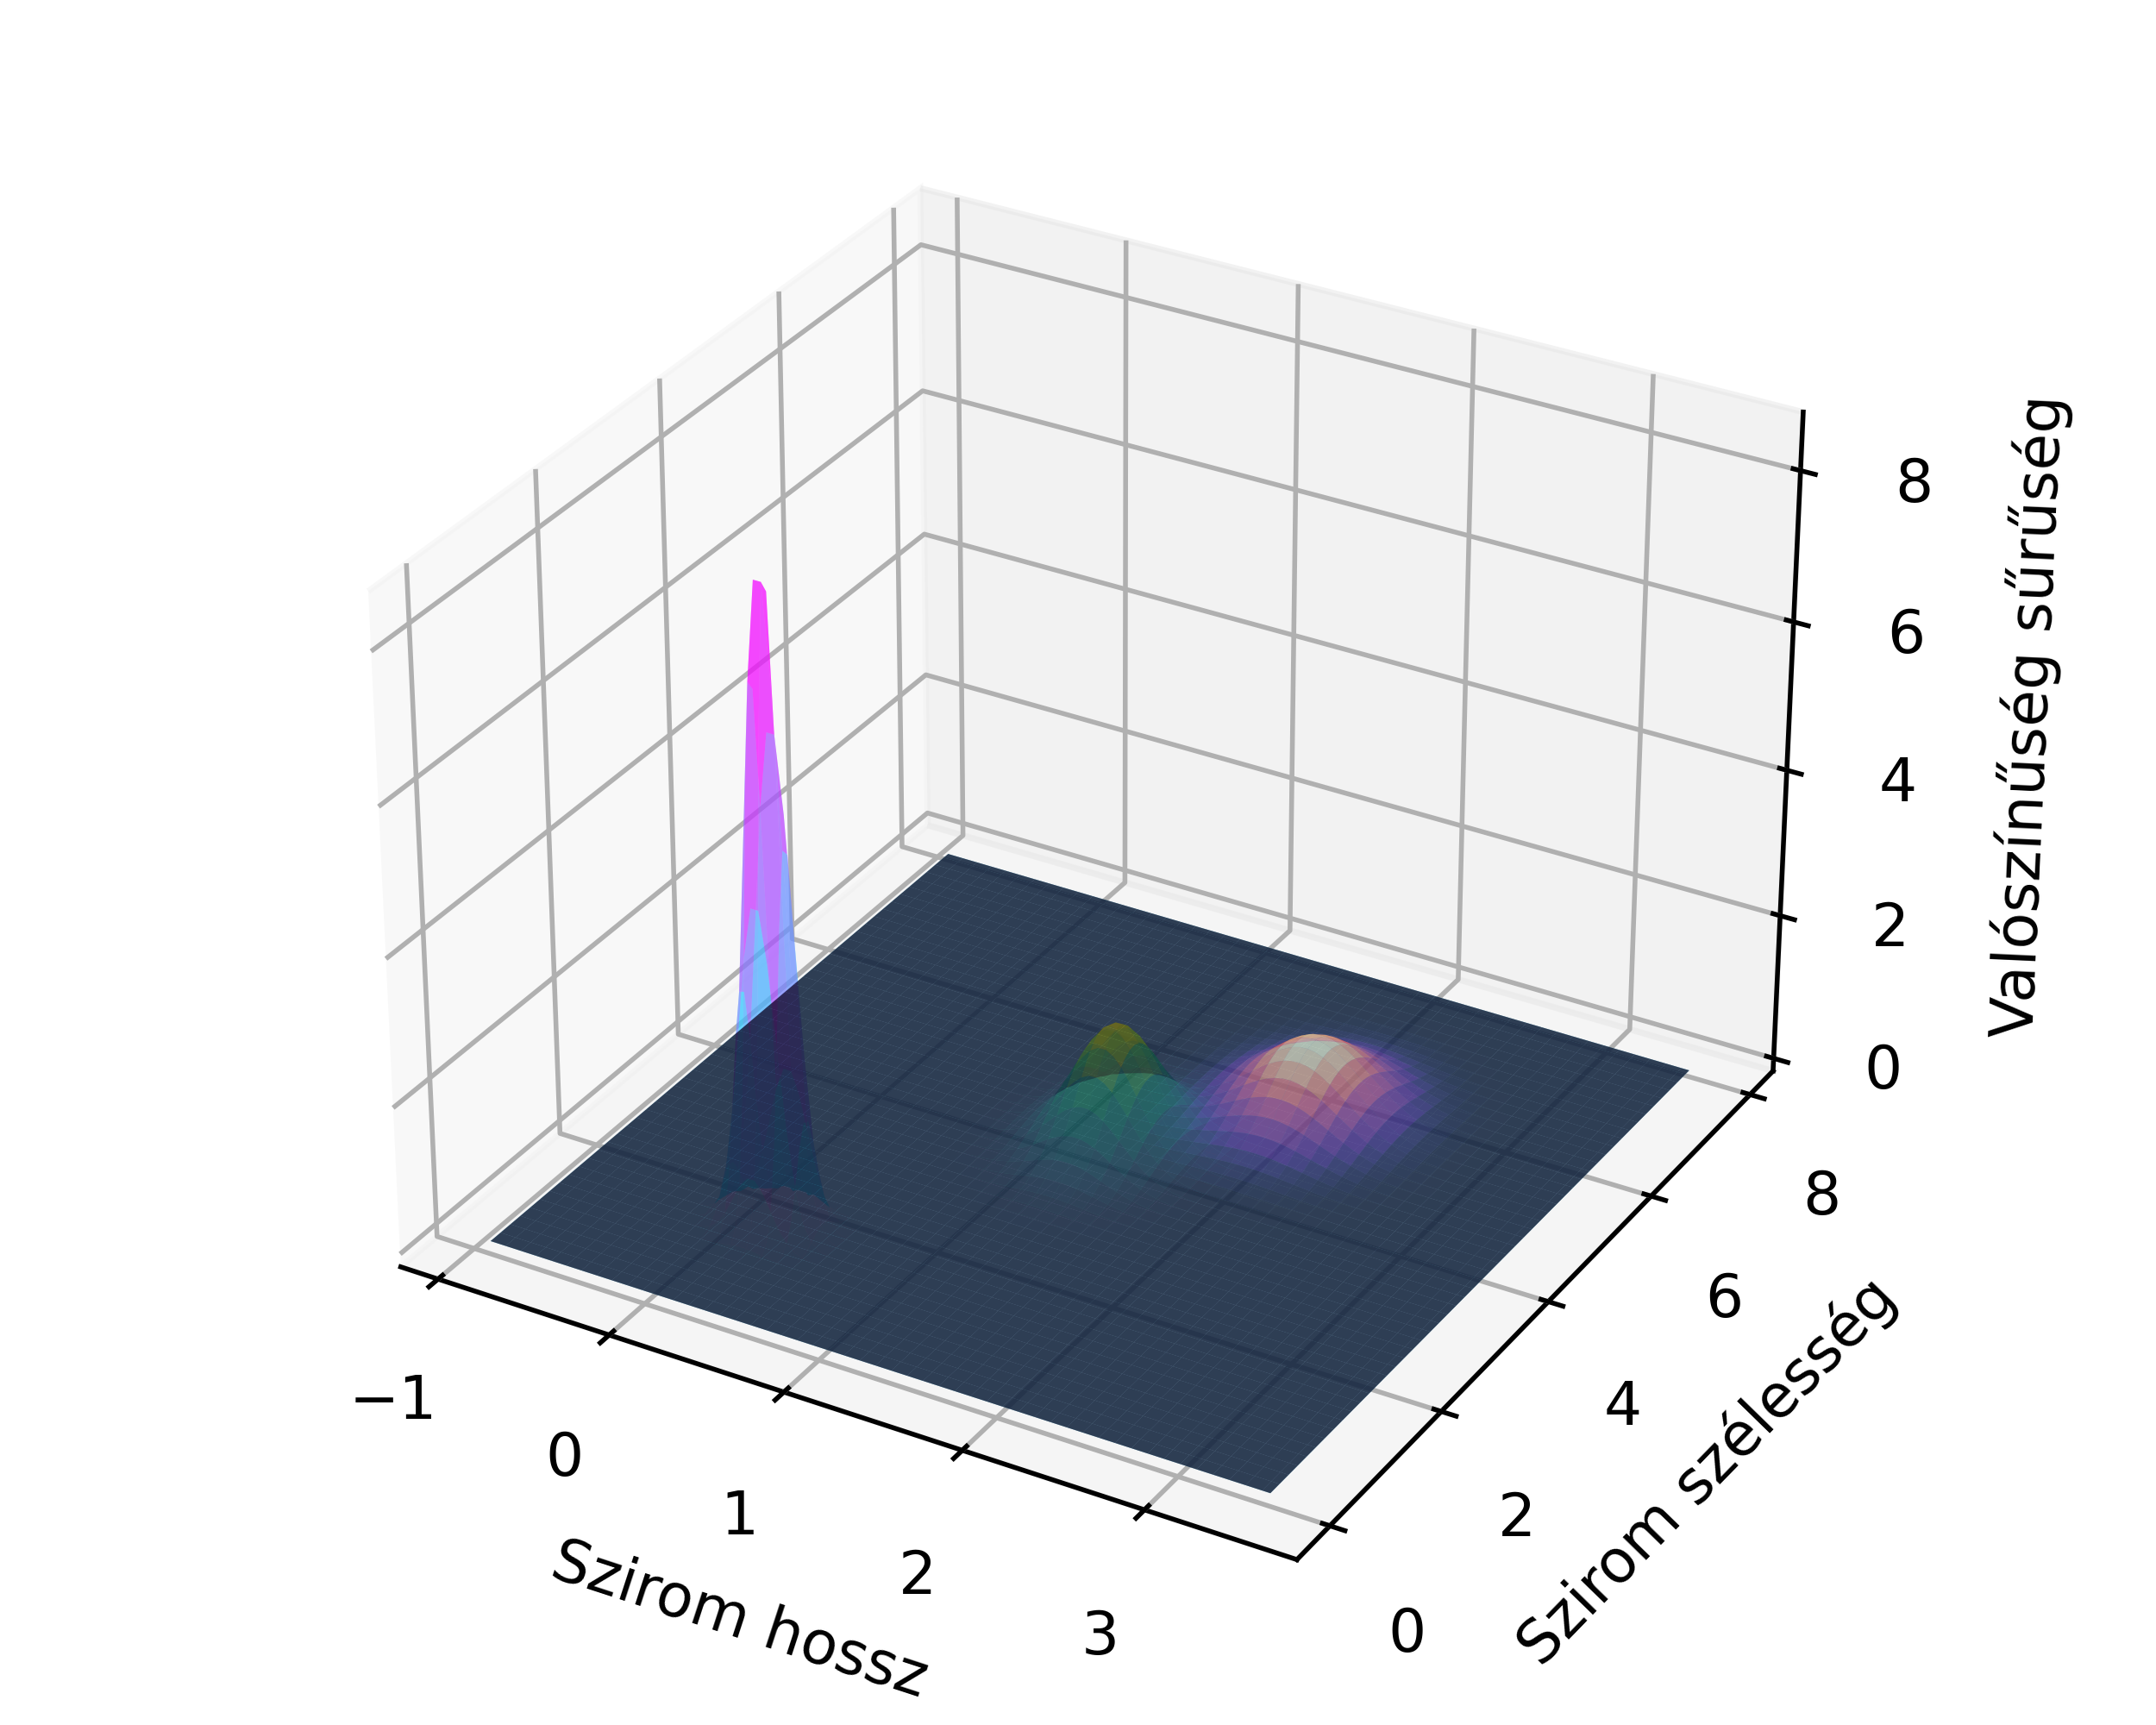
\includegraphics[width=7cm, height=7cm, keepaspectratio]{images/generative_4.png}
\end{center}
\end{column}
\end{columns}
\end{frame}

\begin{frame}{Gauss-i naív Bayes}
\begin{columns}
\begin{column}{.5\textwidth}
A paraméterek becslése a tanító adathalmazra:
\begin{itemize}
	\item A várható érték $\mu_{i,j}$ az $i$ jellemző átlaga minden olyan egyedre, amely $j$ osztályba tartozik
	\item A kovariancia mátrix $\Sigma$ a várható értéktől való négyzetes eltéréseket tartalmazza minden $i,j$ esetén
\end{itemize}
A predikció minden $C_j$ osztály utólagos valószínűsége a Bayes tételnek megfelelően: 
\begin{block}{}
\vspace{-.4cm}
\[
P\left( C_j \vert x_{1 \ldots n} \right) = \frac{P(C_j) \prod_{i=1}^{n} P(x_i | C_j)}{P(x_1, \ldots, x_n)}
\]
\end{block}
\end{column}
\begin{column}{.5\textwidth}
\begin{center}
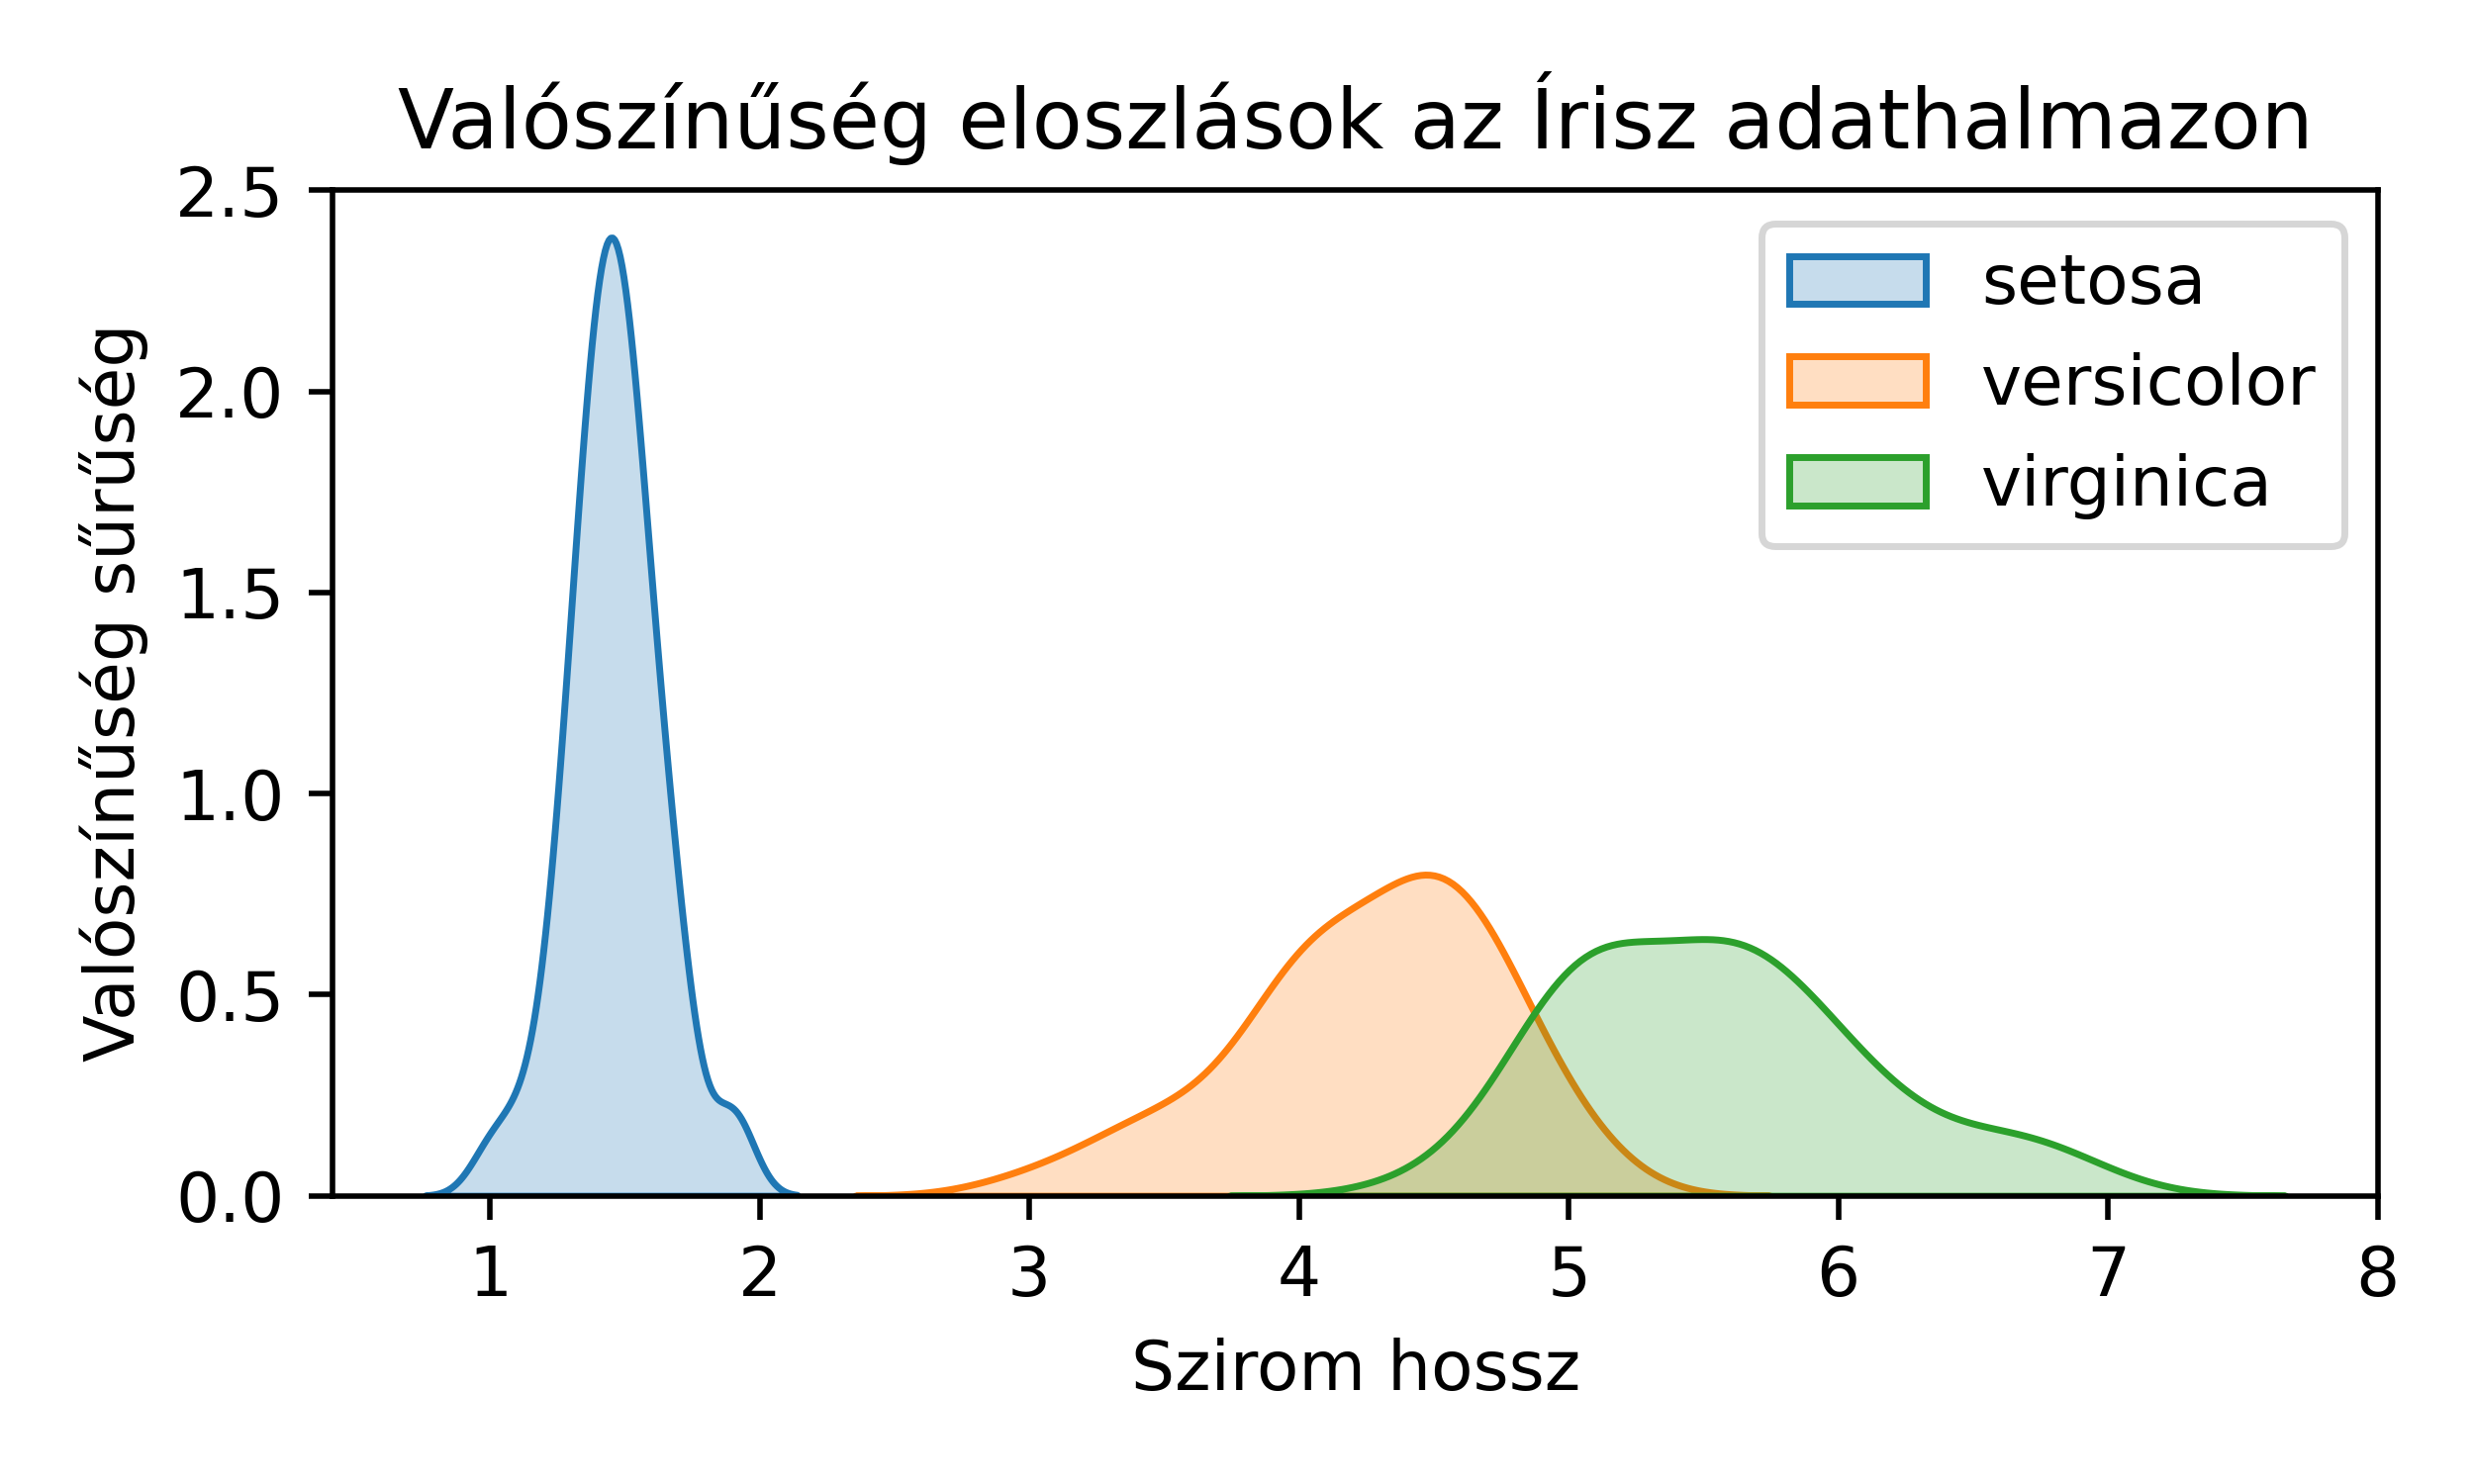
\includegraphics[width=7cm, height=7cm, keepaspectratio]{images/generative_11.png}
\end{center}
\end{column}
\end{columns}
\end{frame}

\section{Gauss-i keverékek}

\begin{frame}
\tableofcontents[currentsection]
\end{frame}

\begin{frame}{Gauss-i keverékek}
\begin{columns}
\begin{column}{.5\textwidth}
Probabilisztikus modellezési eljárás melynek alap feltételezése, hogy \textbf{az adatok ismeretlen paraméterű Gauss-i eloszlások által lettek generálva}.\par\smallskip
Az eljárás megadja, hogy milyen komplex eloszlásból származhatna az adatkészlet, ha véletlen minta lenne.\par\smallskip
A modell célja megkeresni a Gauss-eloszlások $\mu$ és $\Sigma$ paramétereit.
\end{column}
\begin{column}{.5\textwidth}
\begin{center}
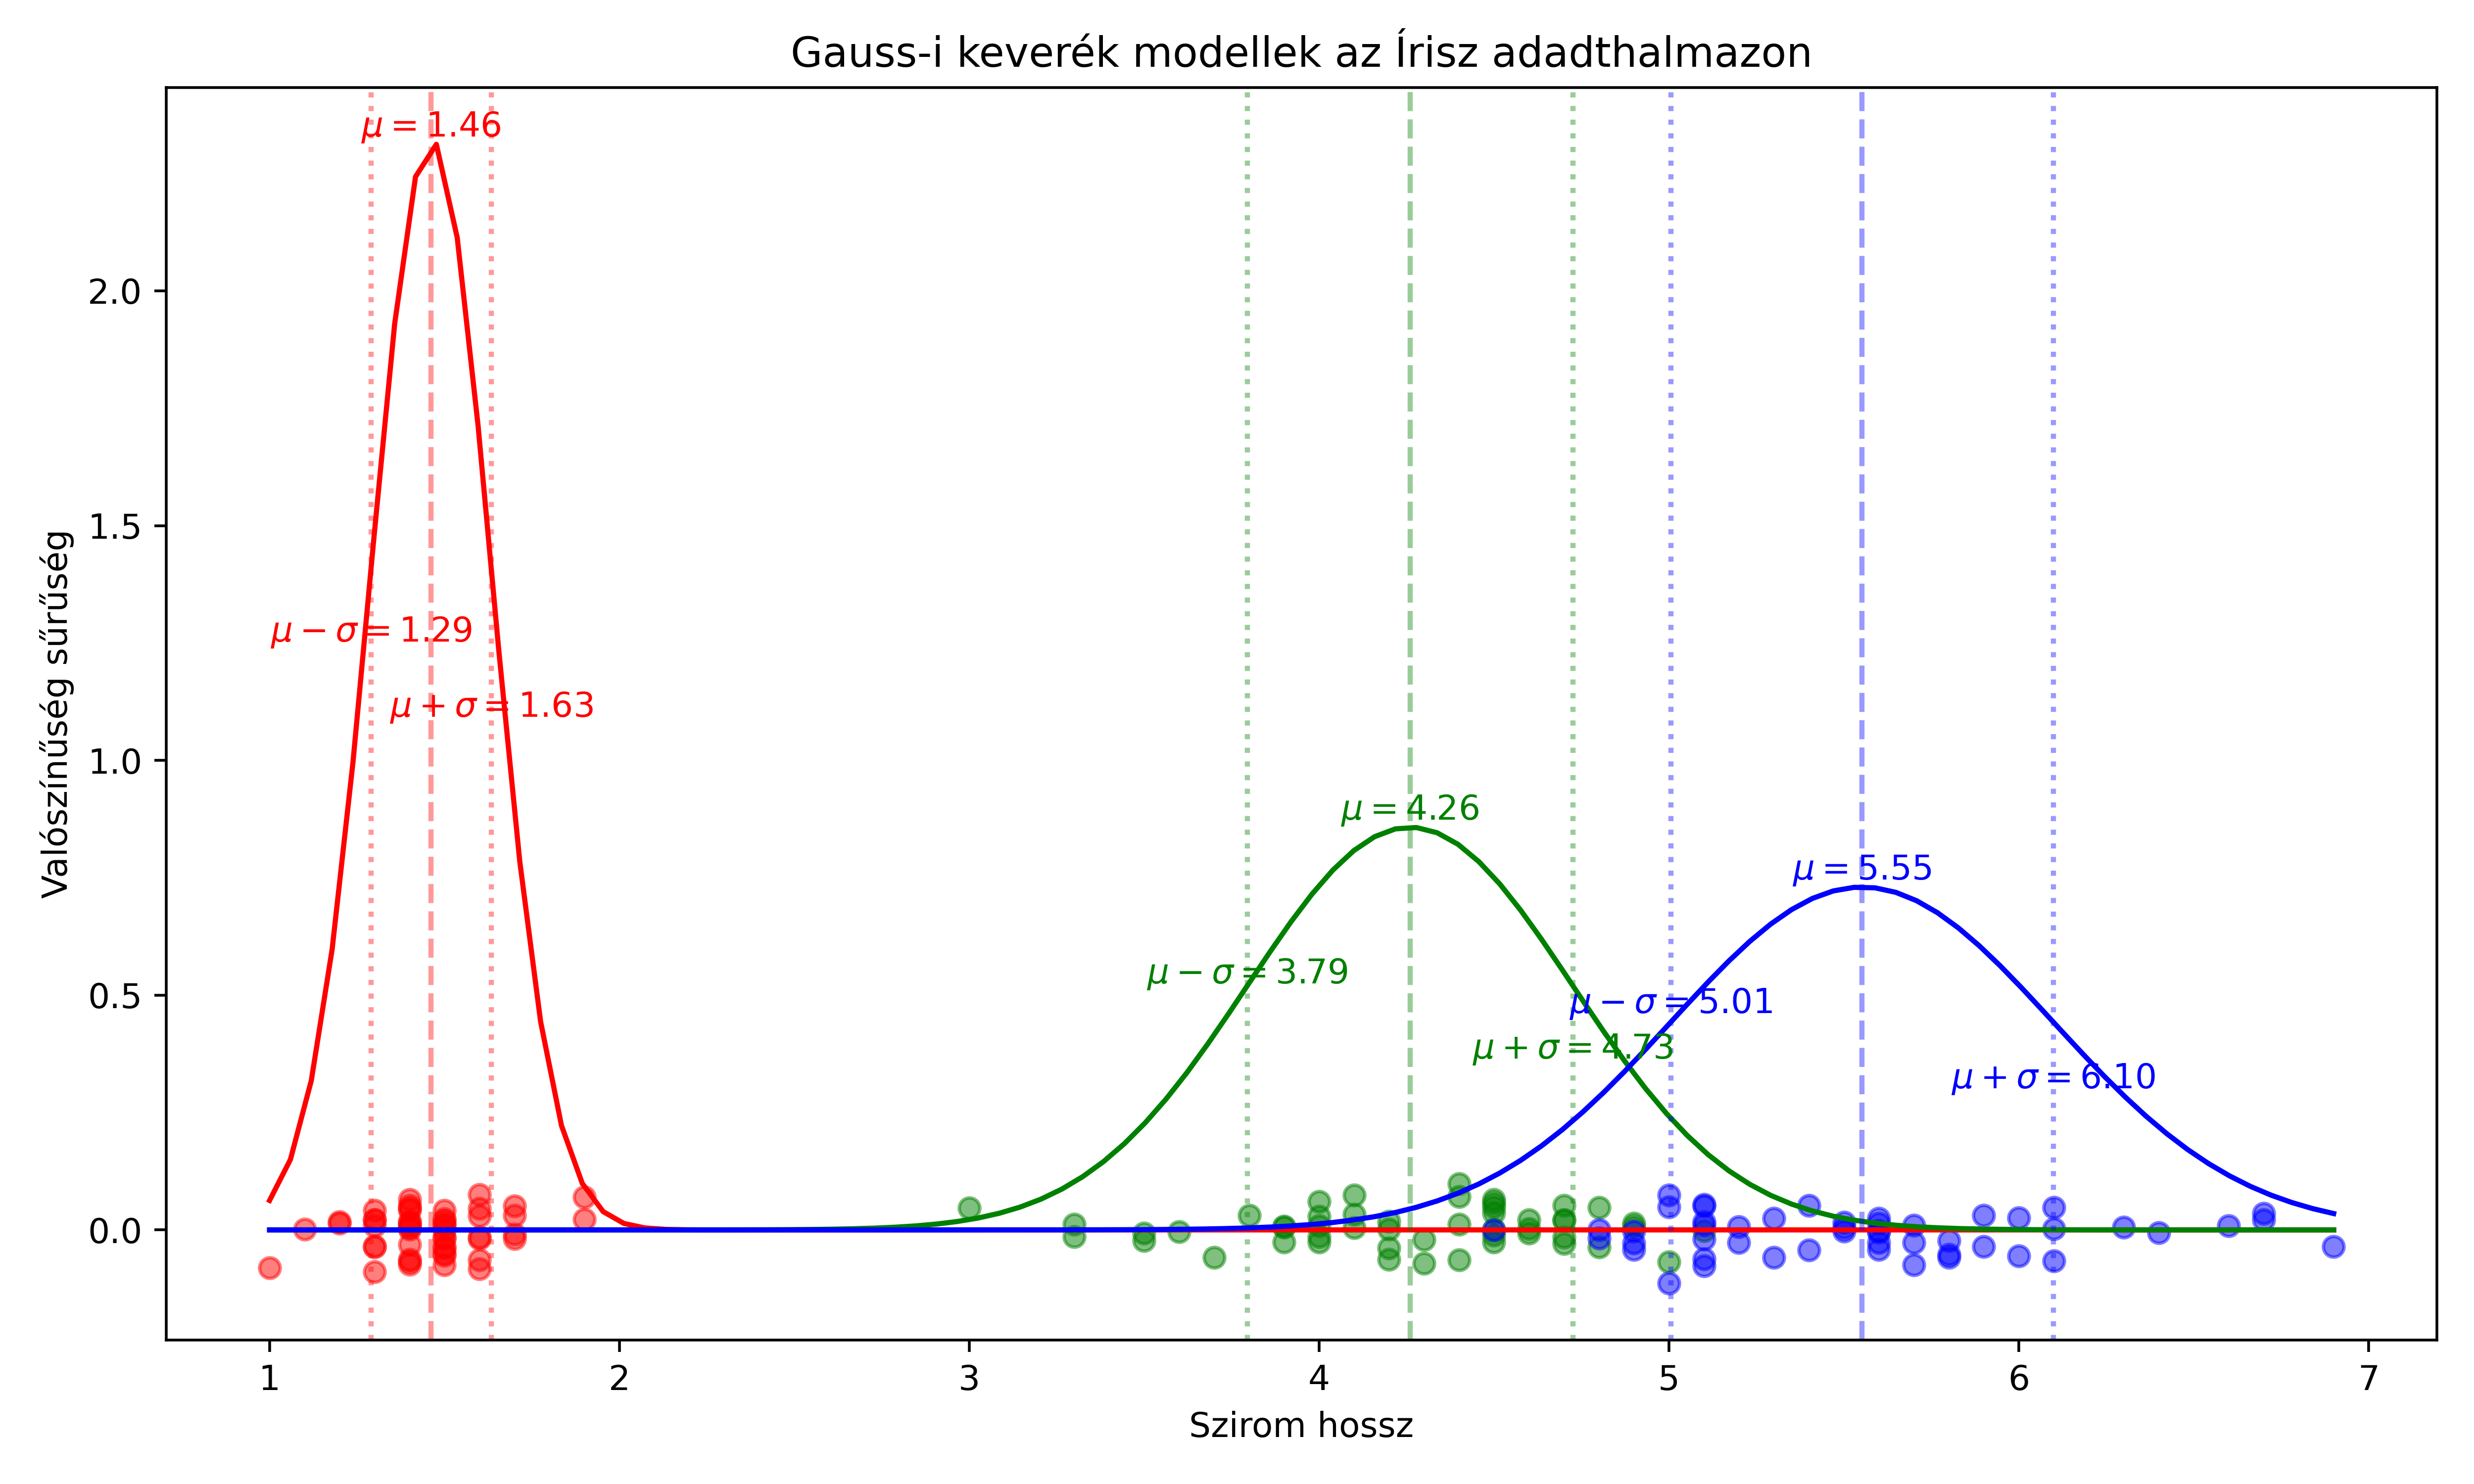
\includegraphics[width=7cm, height=7cm, keepaspectratio]{images/generative_12.png}
\end{center}
\end{column}
\end{columns}
\end{frame}

\begin{frame}{A modellezési eljárás}
\begin{columns}
\begin{column}{.5\textwidth}
A Gauss-i keverékek modellje az EM (elvárás-maximalizálás) algoritmus alapján keresi meg az eloszlások paramétereit:
\begin{enumerate}
	\item \textbf{Inicializáció}: Gauss komponensek számának kiválasztása és véletlenszerű paraméter inicializáció
	\item \textbf{Elvárás}: Felelősségek kiszámítása, amely az a valószínűség minden adatpontra, hogy melyik Gausz komponensből származnak
	\item \textbf{Maximalizálás}: Gauss paraméterek frissítése a valószínűségek maximalizálására, új várható értékek és kovarianciamátrixok kiszámítása
\end{enumerate}
\end{column}
\begin{column}{.5\textwidth}
\begin{center}
\includegraphics<1>[width=7cm, height=7cm, keepaspectratio]{images/generative_13.png}
\includegraphics<2>[width=7cm, height=7cm, keepaspectratio]{images/generative_14.png}
\includegraphics<3>[width=7cm, height=7cm, keepaspectratio]{images/generative_15.png}
\includegraphics<4>[width=7cm, height=7cm, keepaspectratio]{images/generative_16.png}
\includegraphics<5>[width=7cm, height=7cm, keepaspectratio]{images/generative_17.png}
\end{center}
\end{column}
\end{columns}
\end{frame}

\begin{frame}{Az eljárás modellje}
\begin{columns}
\begin{column}{.5\textwidth}
Minden adatponthoz véletlenszerűen rendelődik klaszter $k$ klaszterből. A $j$ klaszter választásának valószínűsége $\phi$. Az $i$ mintaegyedhez rendelt klaszter $z_i$.\par\medskip
Ha $z_i=j$ az $i$ mintaegyed pozíciója szerint $x_i$ véletlen minta választódik ki abból a Gauss eloszlásból $\mu, \Sigma$ paraméterekkel: $x_i \sim N\left( \mu_j, \Sigma_j \right)$, azaz a $P\left( x_i \vert z_i = k, \mu_k, \Sigma_k \right)$ valószínűség.\par\medskip
A körök véletlen változók és a téglalapok fix értékek. 
\end{column}
\begin{column}{.5\textwidth}
\begin{center}
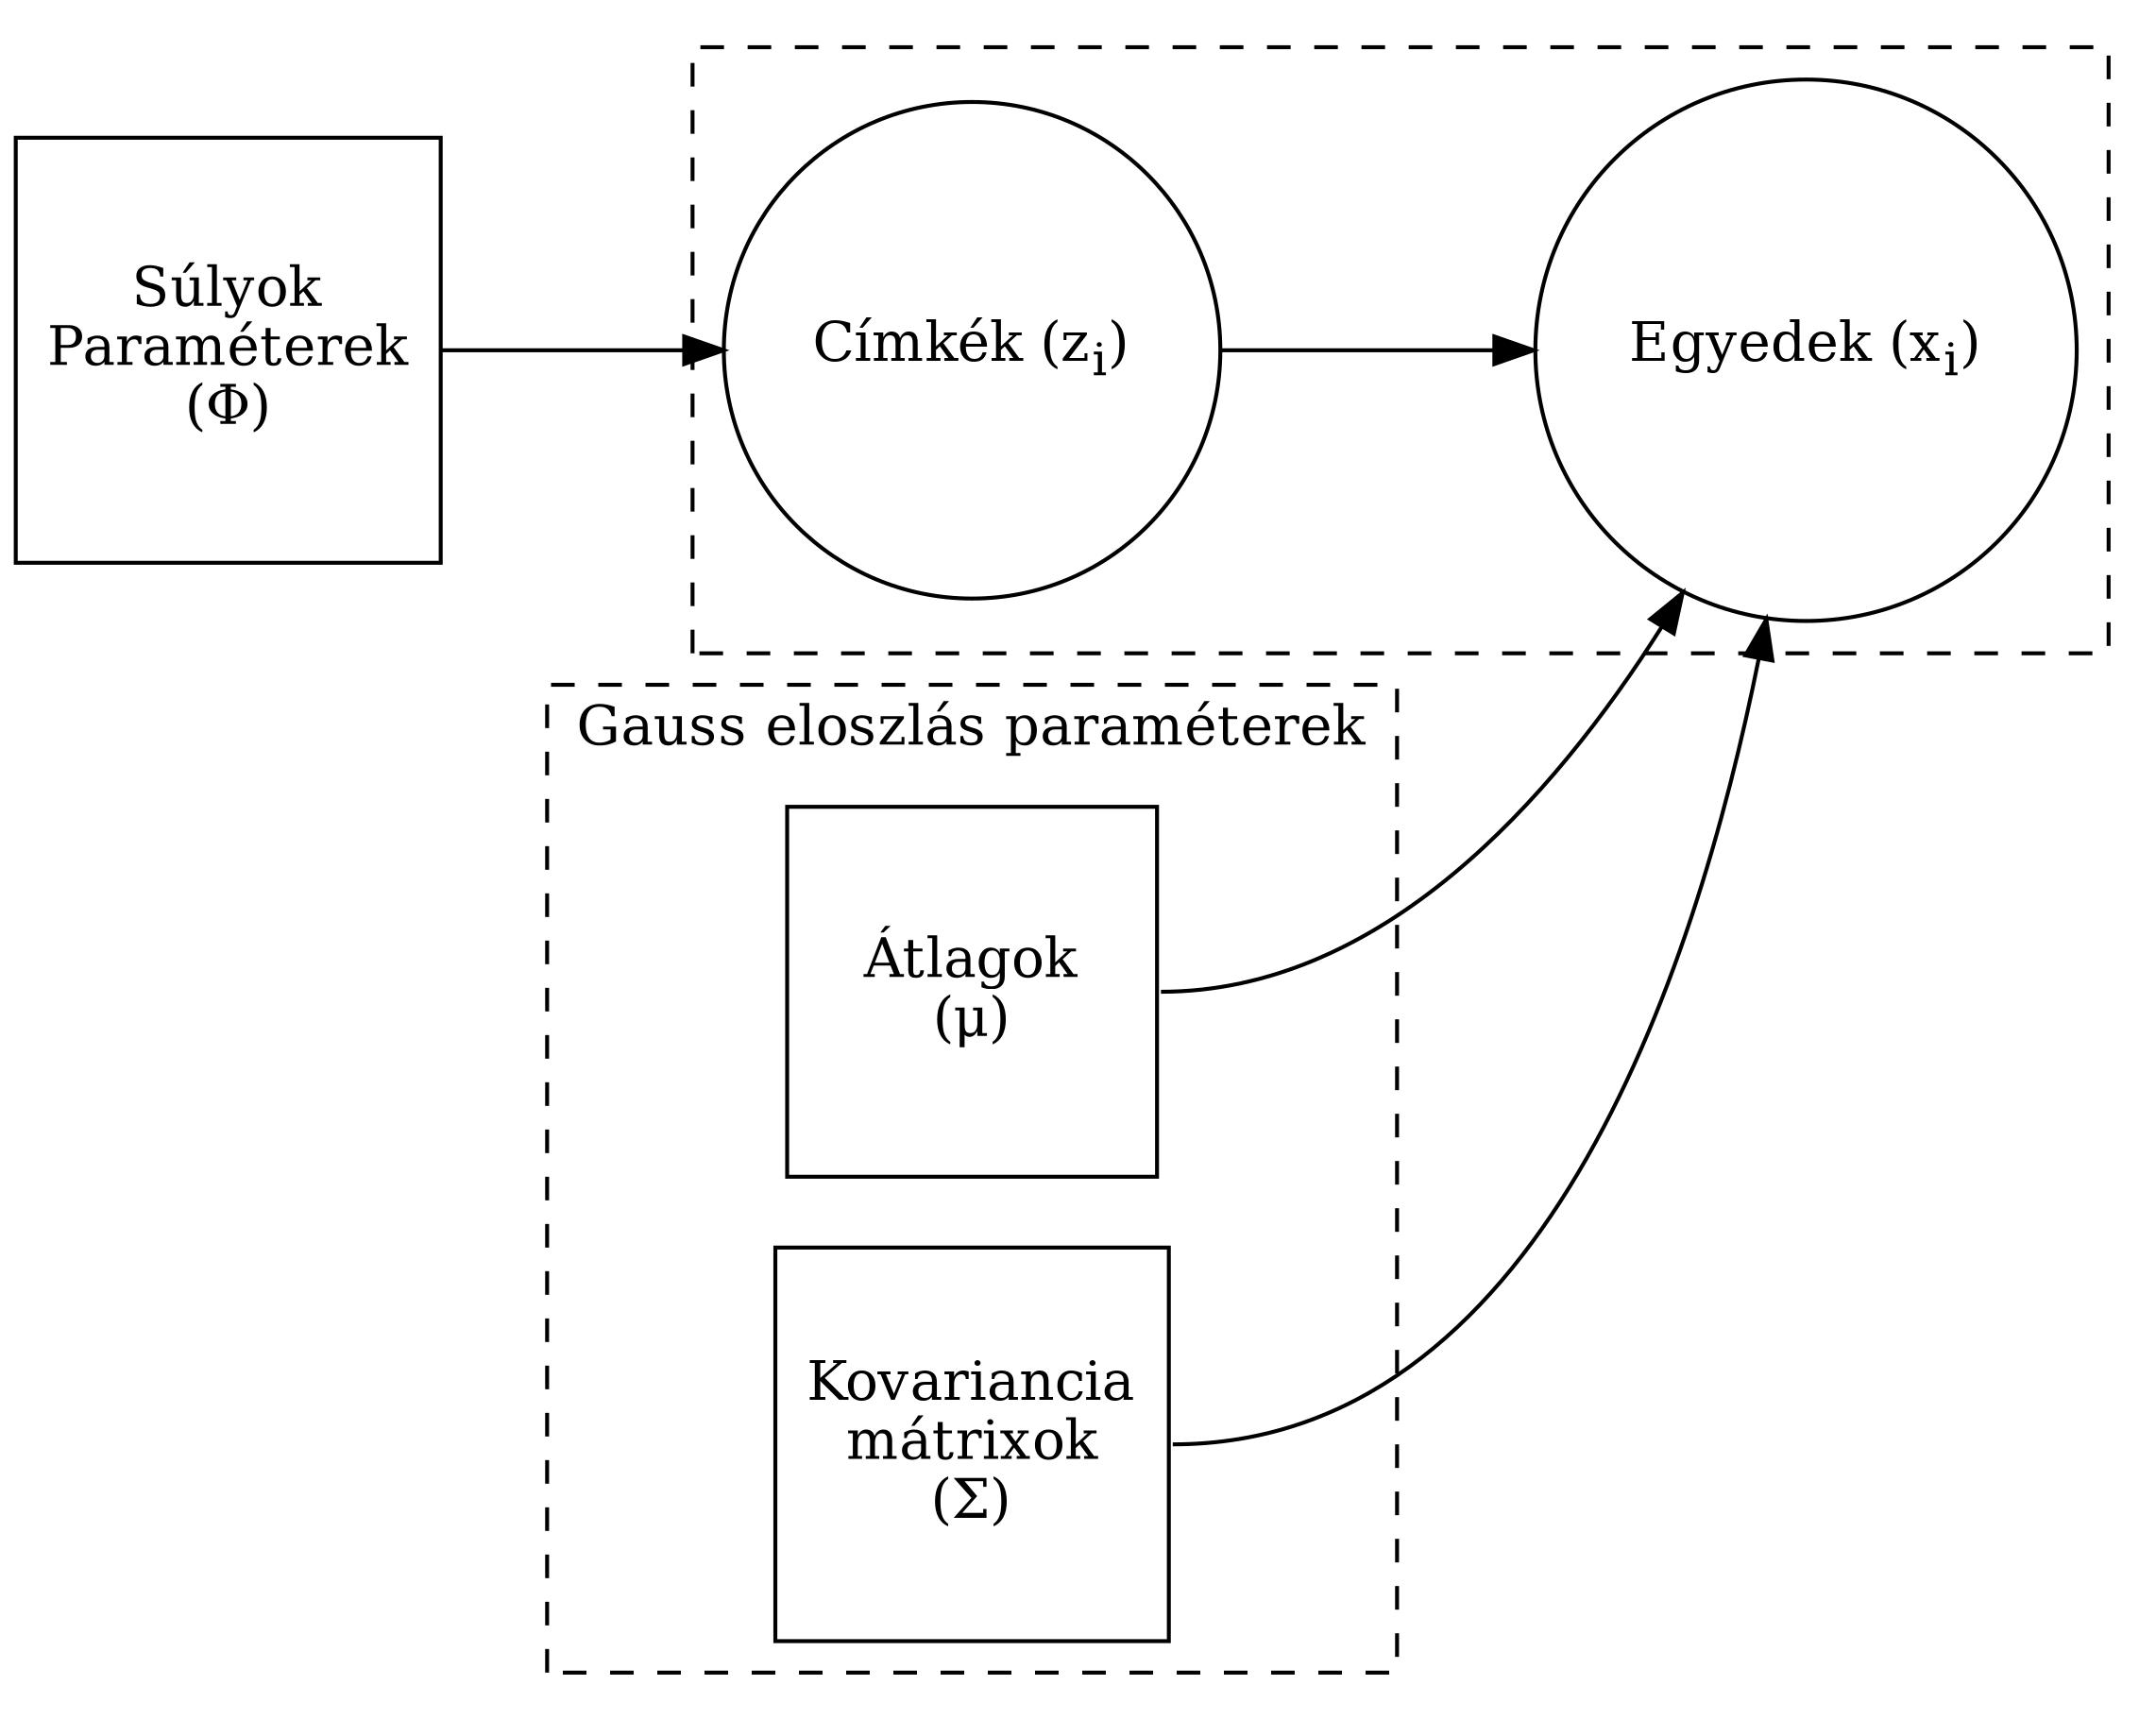
\includegraphics[width=7cm, height=7cm, keepaspectratio]{graphs/generative_4.png}
\end{center}
\end{column}
\end{columns}
\end{frame}

\begin{frame}{A Gauss-i keverékek és $K$-közép kapcsolata}
\begin{columns}
\begin{column}{.5\textwidth}
Az EM algoritmus a $K$-közép generalizált változata, ami nem csak a centroidokat keresi meg, hanem a klaszterek méretét, orientációját és a relatív súlyaikat is.\par\smallskip
\begin{center}
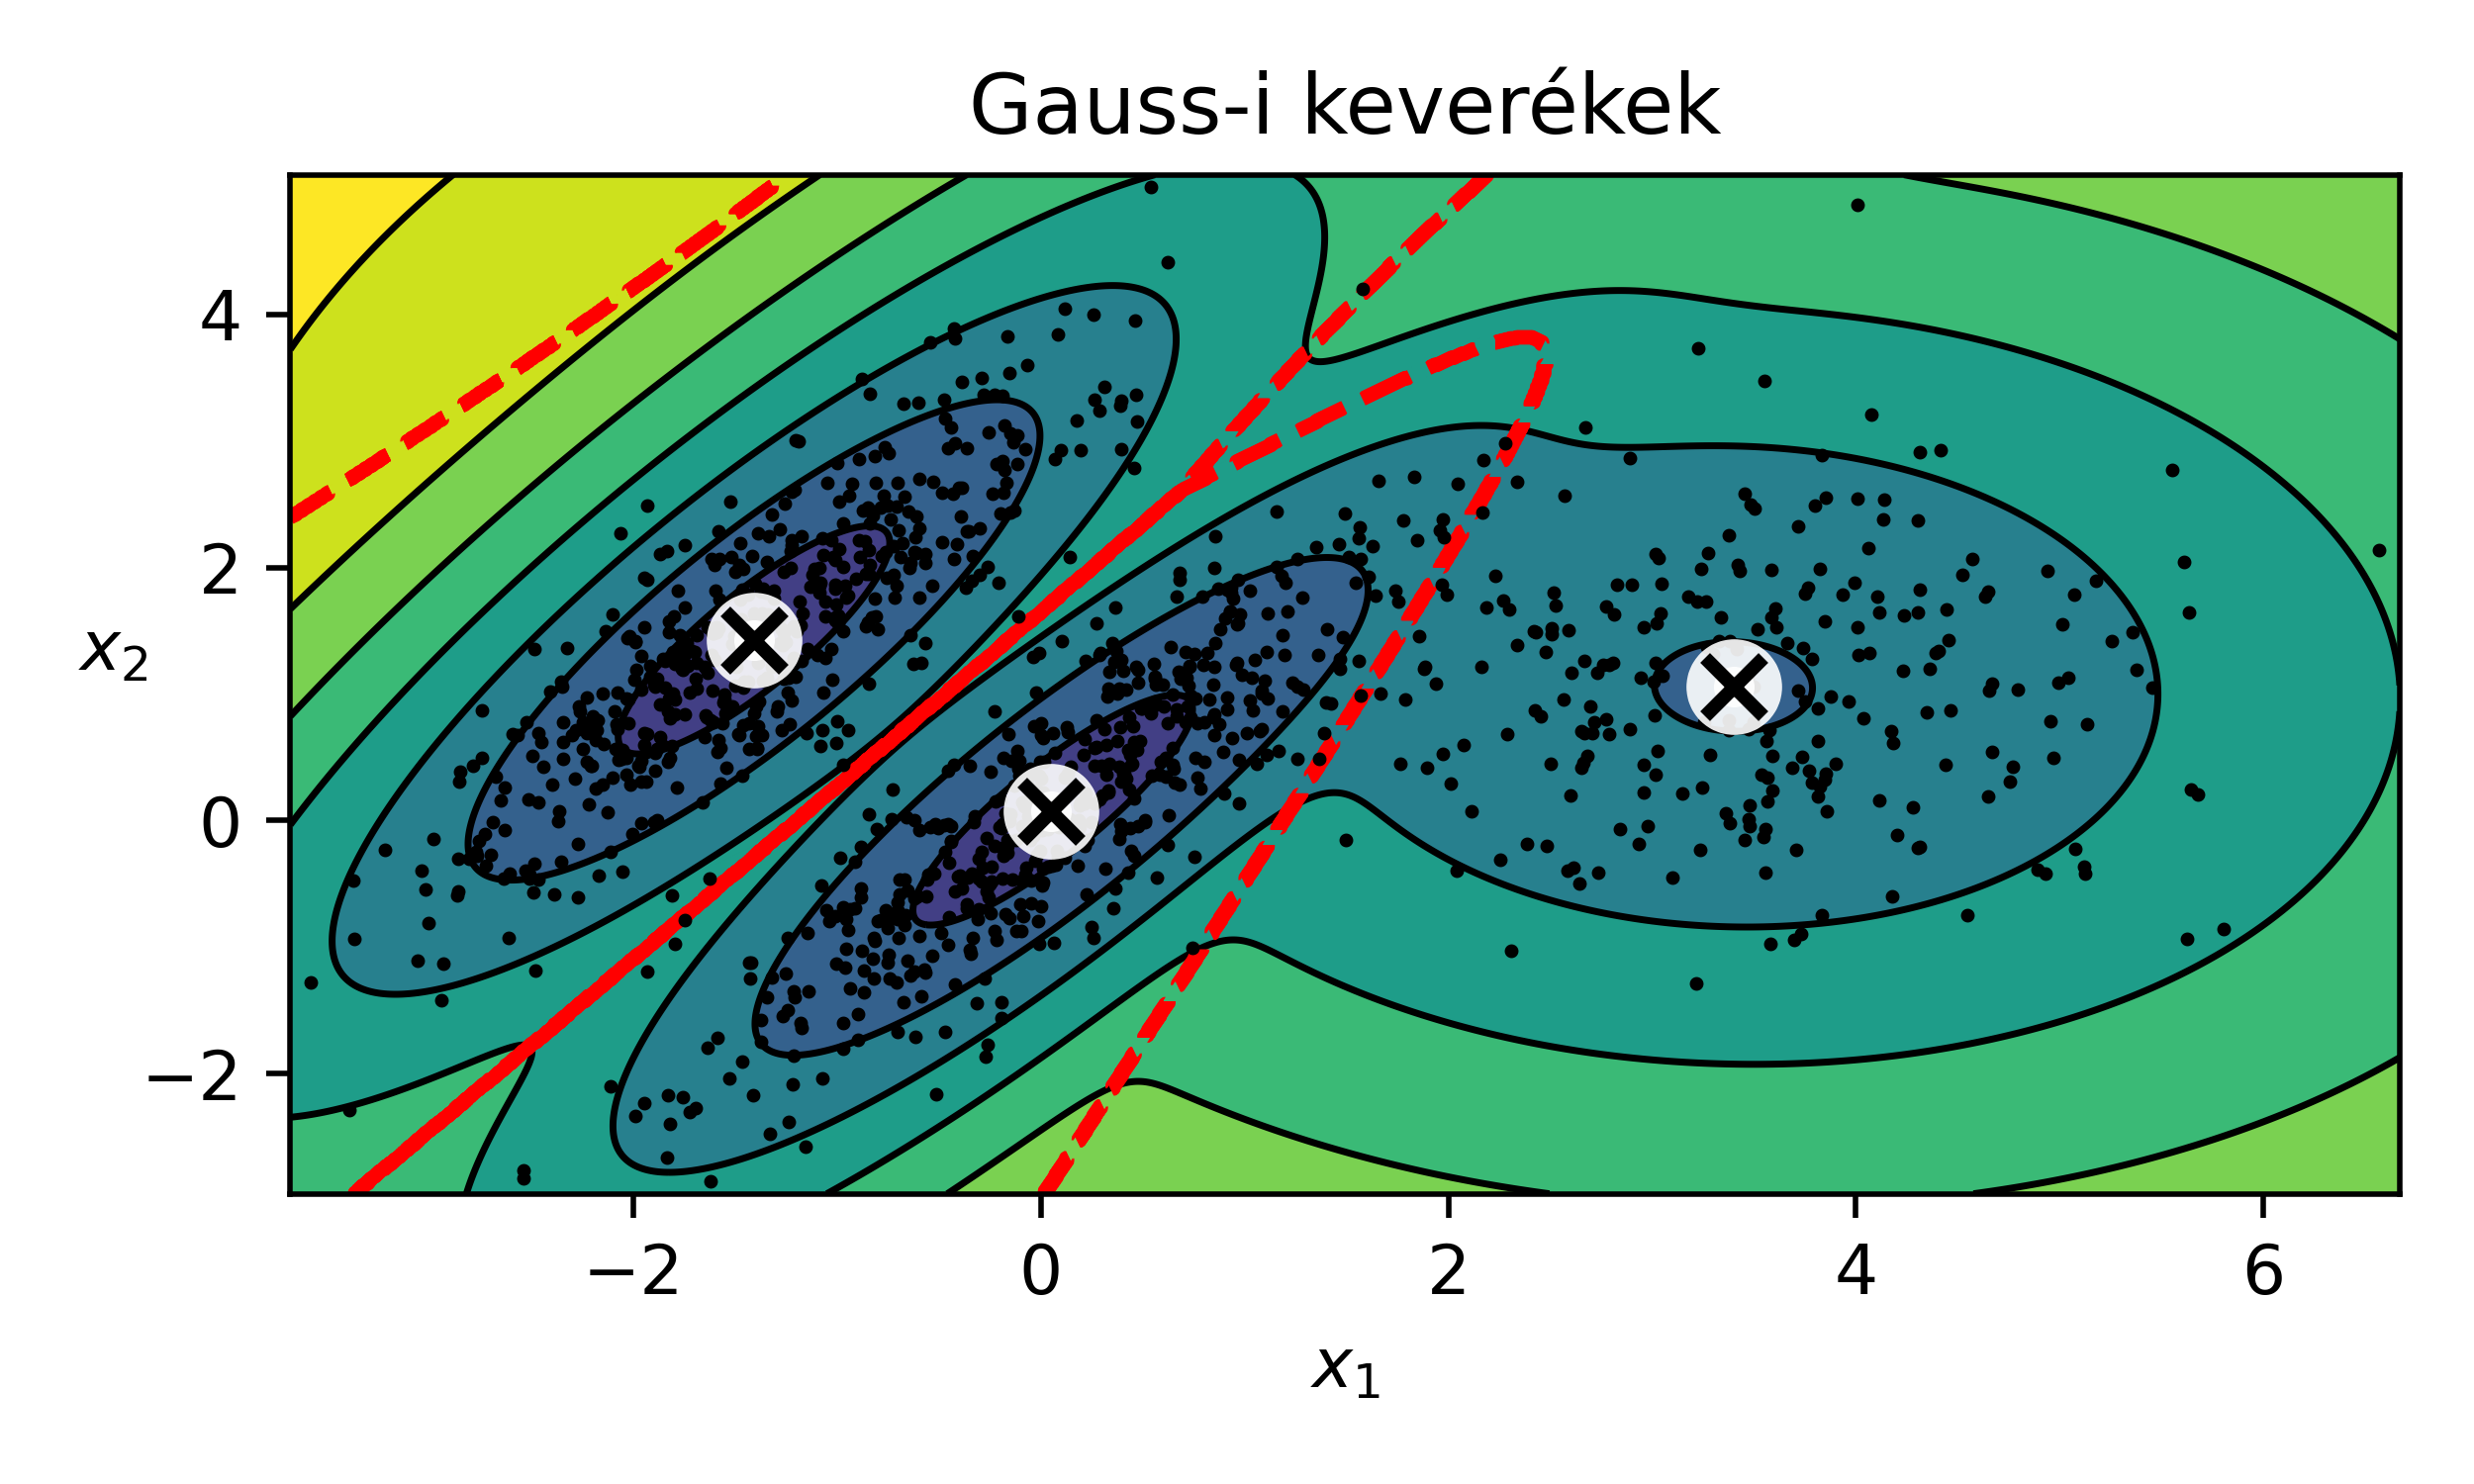
\includegraphics[width=7cm, height=7cm, keepaspectratio]{images/generative_19.png}
\end{center}
\end{column}
\begin{column}{.5\textwidth}
Ezzel sikerül javítania a $K$-közép problémáin amik miatt nem teljesít jól irreguláris sűrűségű, szóródású és formájú klaszterek esetén.
\begin{center}
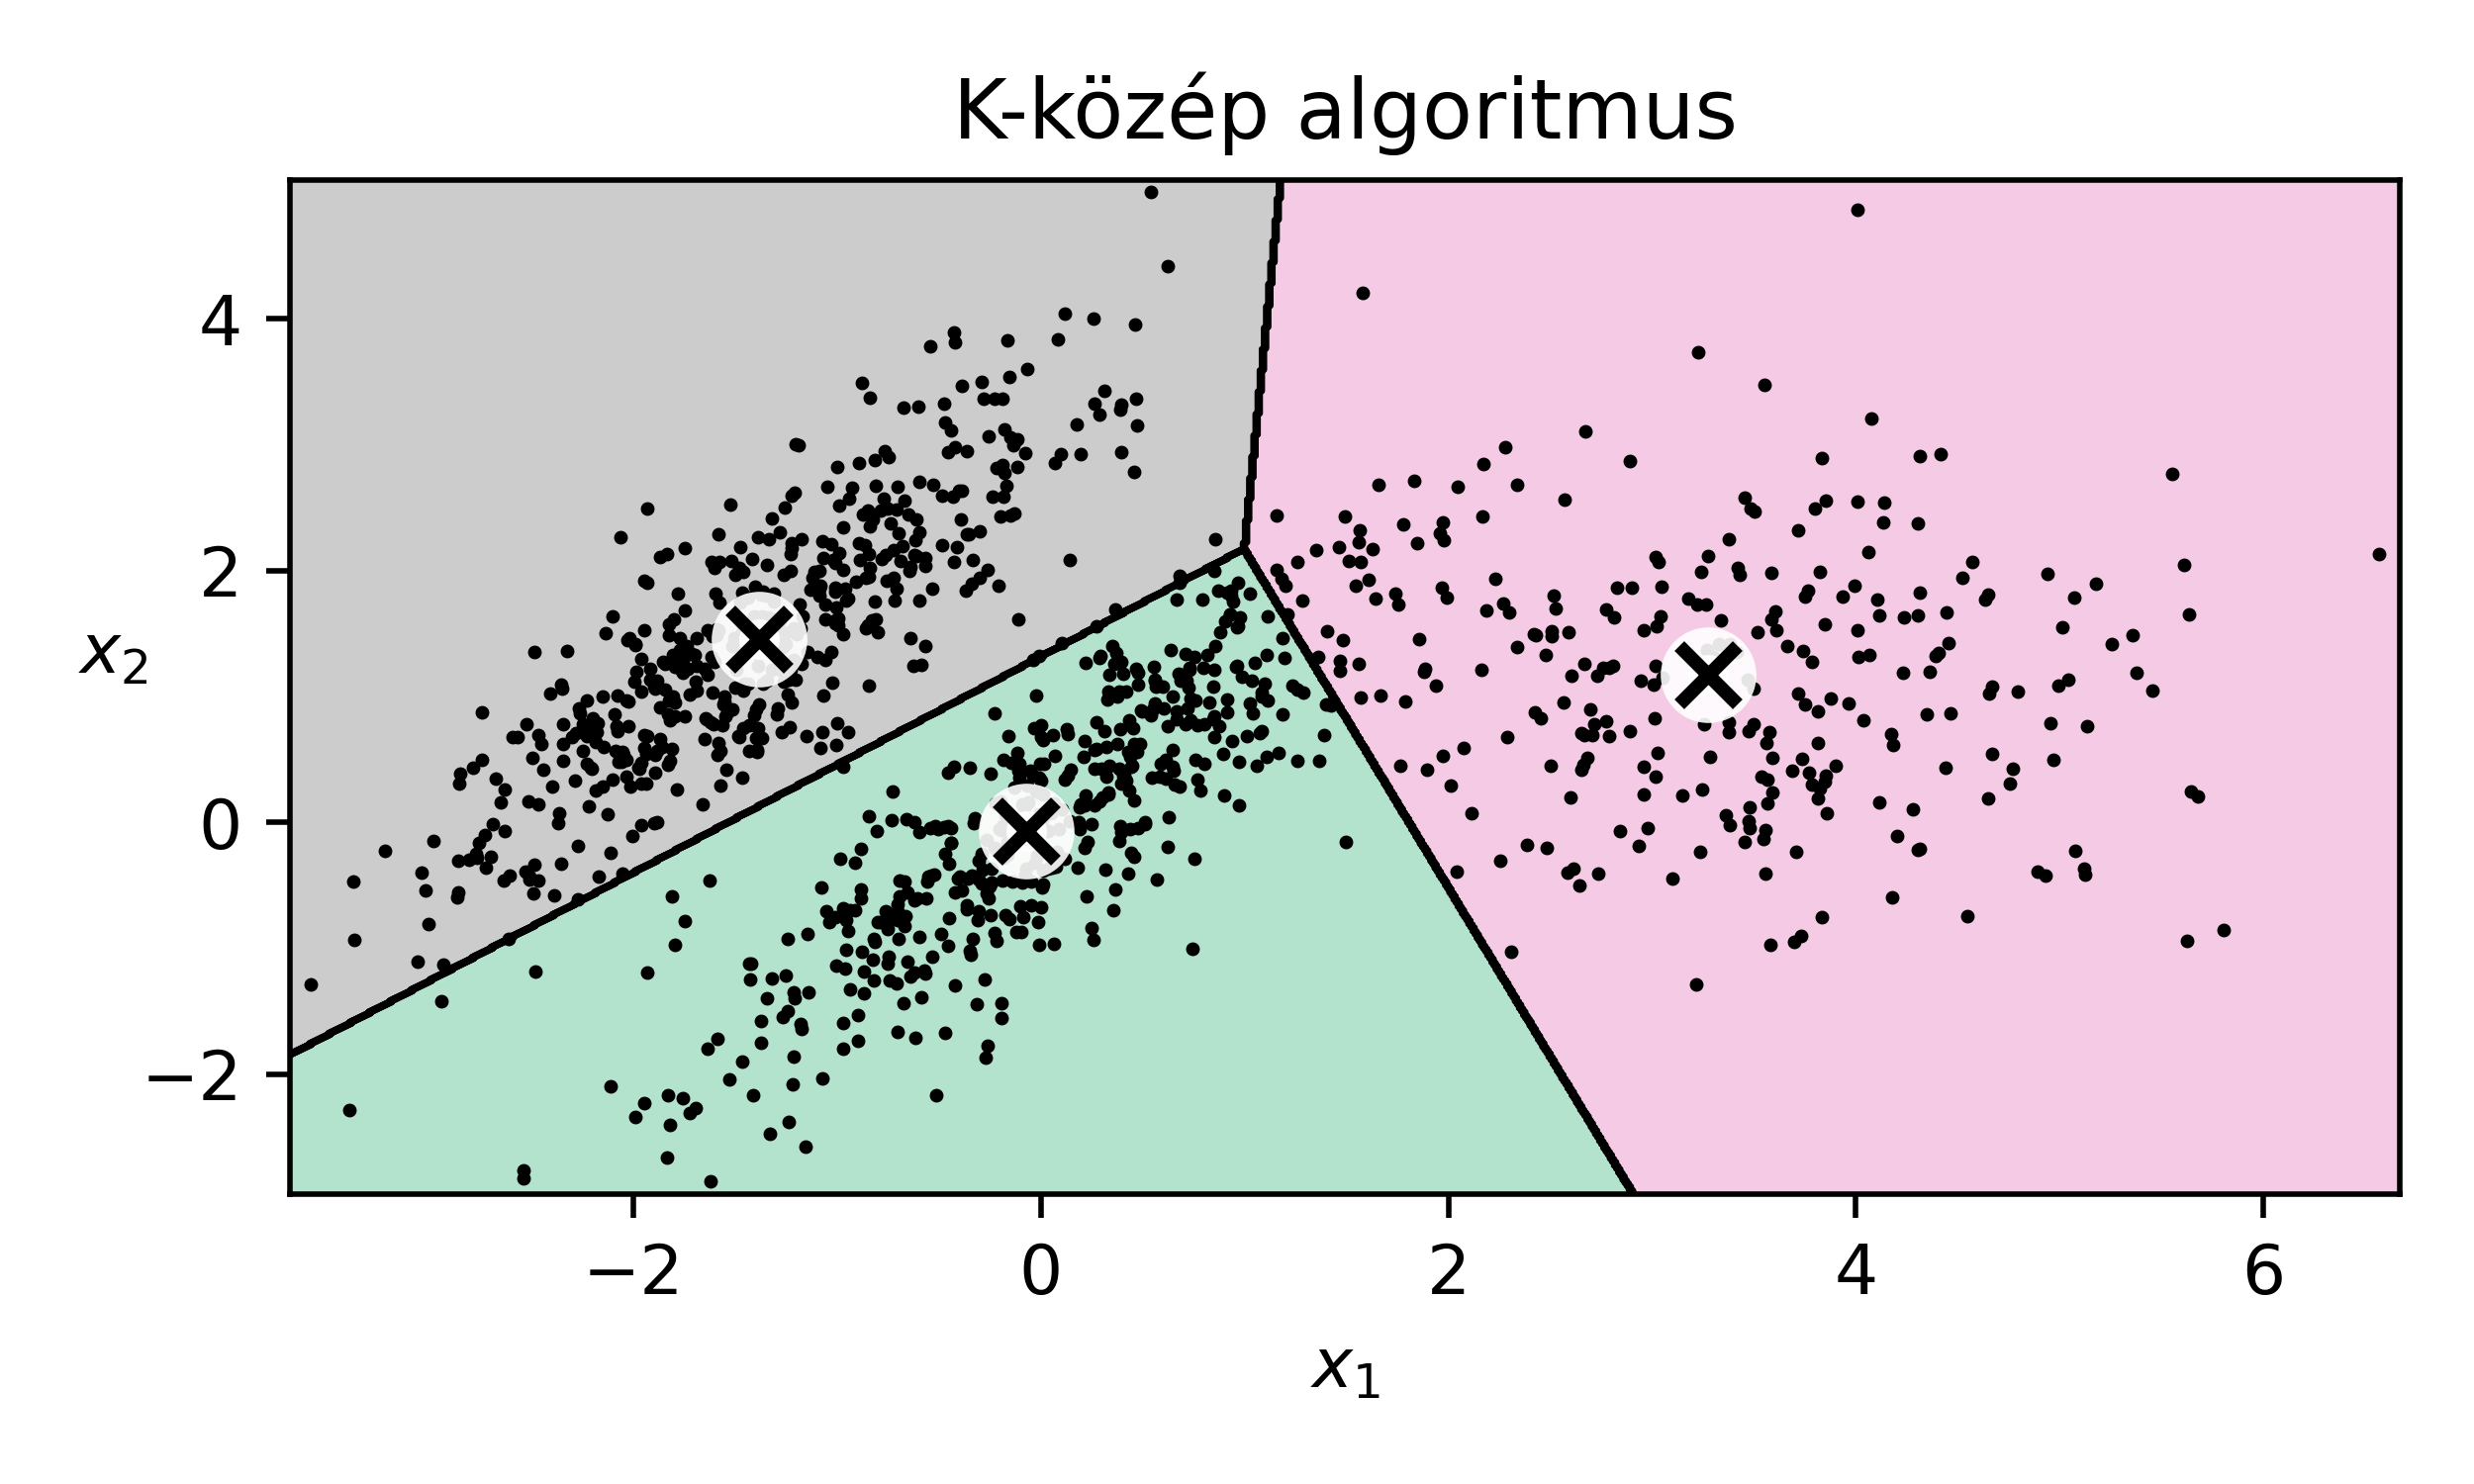
\includegraphics[width=7cm, height=7cm, keepaspectratio]{images/generative_18.png}
\end{center}
\end{column}
\end{columns}
\end{frame}

\begin{frame}{Regularizáció a keverék modellek esetén}
\begin{columns}
\begin{column}{.5\textwidth}
A keverékek esetén a regularizáció a kovariancia mátrixokra tett megkötésekkel érhető el. Ez a \texttt{covariance\_type} paraméter. A lehetséges értékei a következők:\par\medskip
\only<1>{\texttt{spherical}: Kör alakú klaszterek, különböző átmérőkkel (szórással).}
\only<2>{\texttt{diag}: Csak ellipszoid alakú lehet a klaszter, és a tengelyeinek a koordináta-rendszer tengelyeivel párhuzamosnak kell lennie.}
\only<3>{\texttt{tied}: Minden létrejövő klaszternek ugyanolyan formájúnak, méretűnek, és orientációjúnak kell lennie.}
\only<4>{\texttt{full}: Nincs regularizáció.}
\end{column}
\begin{column}{.5\textwidth}
\begin{center}
\includegraphics<1>[width=7cm, height=7cm, keepaspectratio]{images/generative_22.png}
\includegraphics<2>[width=7cm, height=7cm, keepaspectratio]{images/generative_23.png}
\includegraphics<3>[width=7cm, height=7cm, keepaspectratio]{images/generative_21.png}
\includegraphics<4>[width=7cm, height=7cm, keepaspectratio]{images/generative_20.png}
\end{center}
\end{column}
\end{columns}
\end{frame}

\begin{frame}{Anomália detekció Gauss-i keverékekkel}
\begin{columns}
\begin{column}{.5\textwidth}
A keverék modellek esetén minden olyan mintaegyed, amelyhez \textbf{adott küszöbnél alacsonyabb valószínűség sűrűség tartozik, anomáliának számít}.\par\smallskip
Ha túlságosan magas az anomáliák aránya, a küszöbértéket csökkenteni kell. Az ábrán a küszöbérték a negyedik percentilis.
\end{column}
\begin{column}{.5\textwidth}
\begin{center}
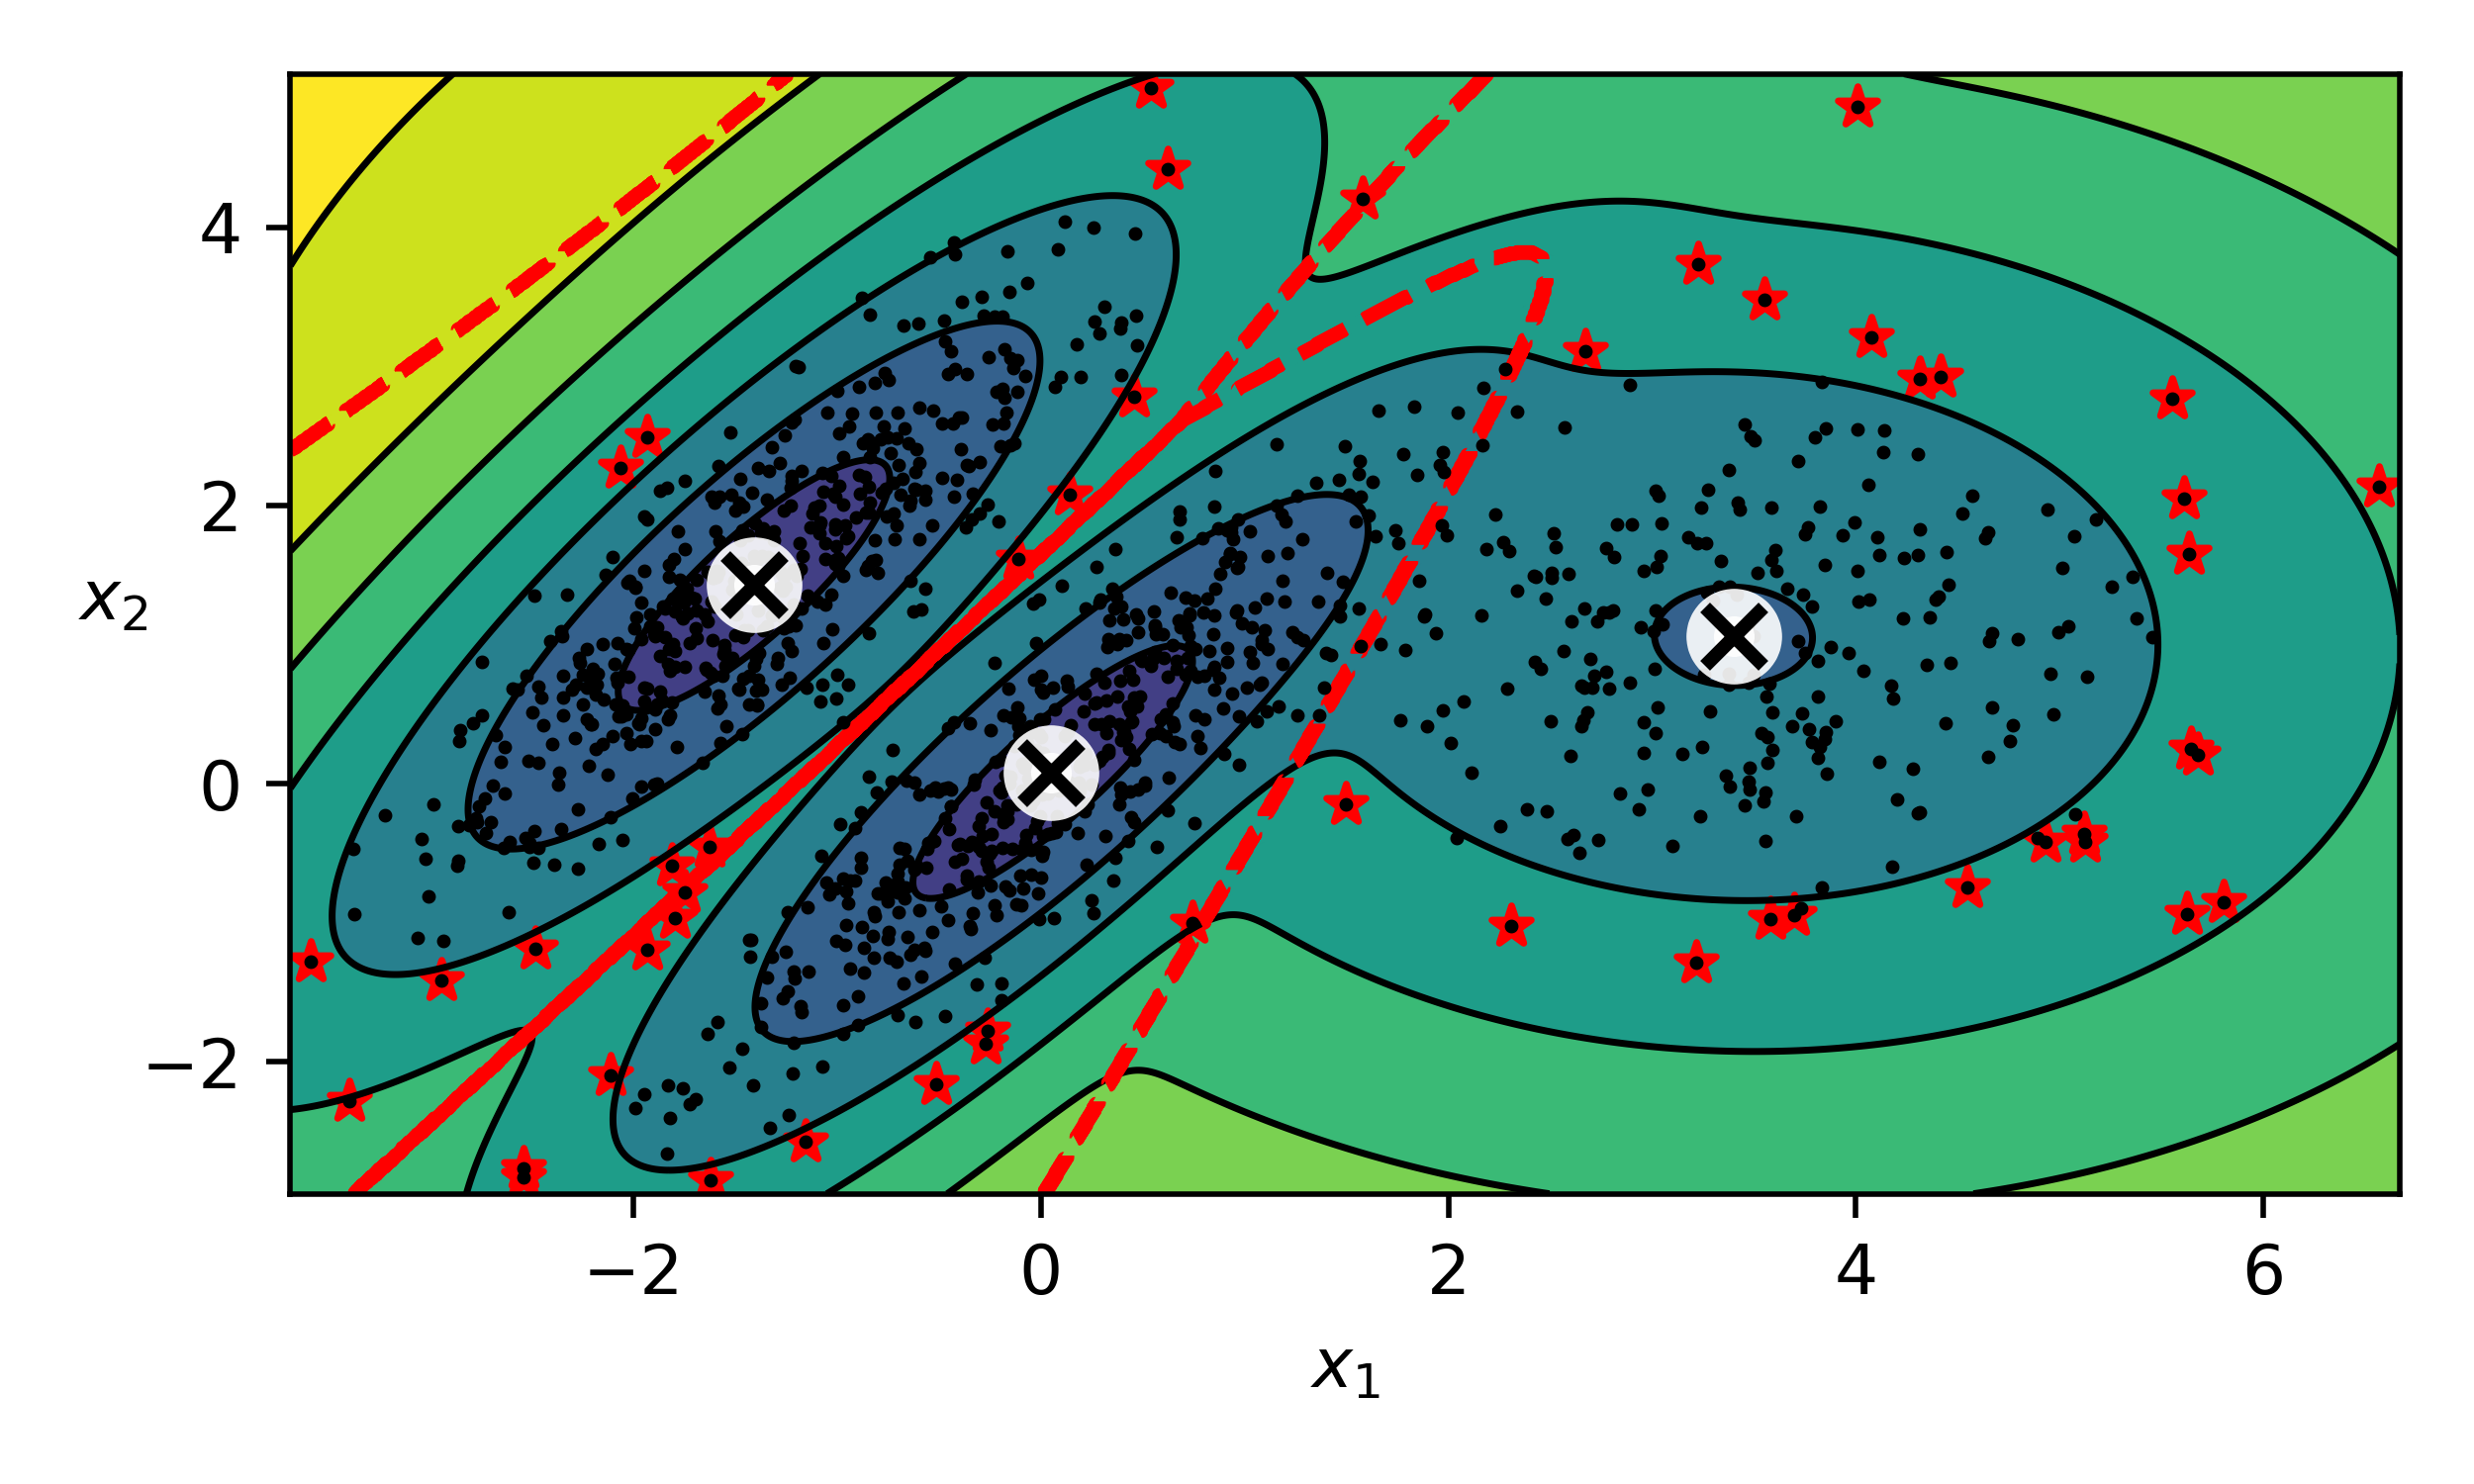
\includegraphics[width=7cm, height=7cm, keepaspectratio]{images/generative_24.png}
\end{center}
\end{column}
\end{columns}
\end{frame}

\begin{frame}{GMM klaszterezésre}
\begin{columns}
\begin{column}{.5\textwidth}
A következő példában a GMM feladata klaszterezni a \texttt{make-moons} által létrehozott irreguláris formájú klasztereket.\par\smallskip
Mivel a GMM nem egy klaszterező algoritmus, \textbf{a két hold alakú klasztert nem képes megfelelően definiálni}. 
\end{column}
\begin{column}{.5\textwidth}
\begin{center}
\includegraphics<1>[width=7cm, height=7cm, keepaspectratio]{images/generative_25.png}
\includegraphics<2>[width=7cm, height=7cm, keepaspectratio]{images/generative_27.png}
\end{center}
\end{column}
\end{columns}
\end{frame}

\begin{frame}{GMM sűrűségek becslésére}
\begin{columns}
\begin{column}{.5\textwidth}
A 2 generátor által definiált klaszter konfiguráció szuboptimális, mert nem képesek megfelelően szeparálni a két holdhoz tartozó klasztert.\par\smallskip
Az ábrán látható, mi történik, ha 2 helyett 10 generátor illeszkedik az adatpontokra.\par\smallskip
\textbf{Ez továbbra sem lesz képes megfelelő módon elvégezni a klaszterezés feladatát, de az adatpontok sűrűségét már jóval pontosabban becsüli meg}. 
\end{column}
\begin{column}{.5\textwidth}
\begin{center}
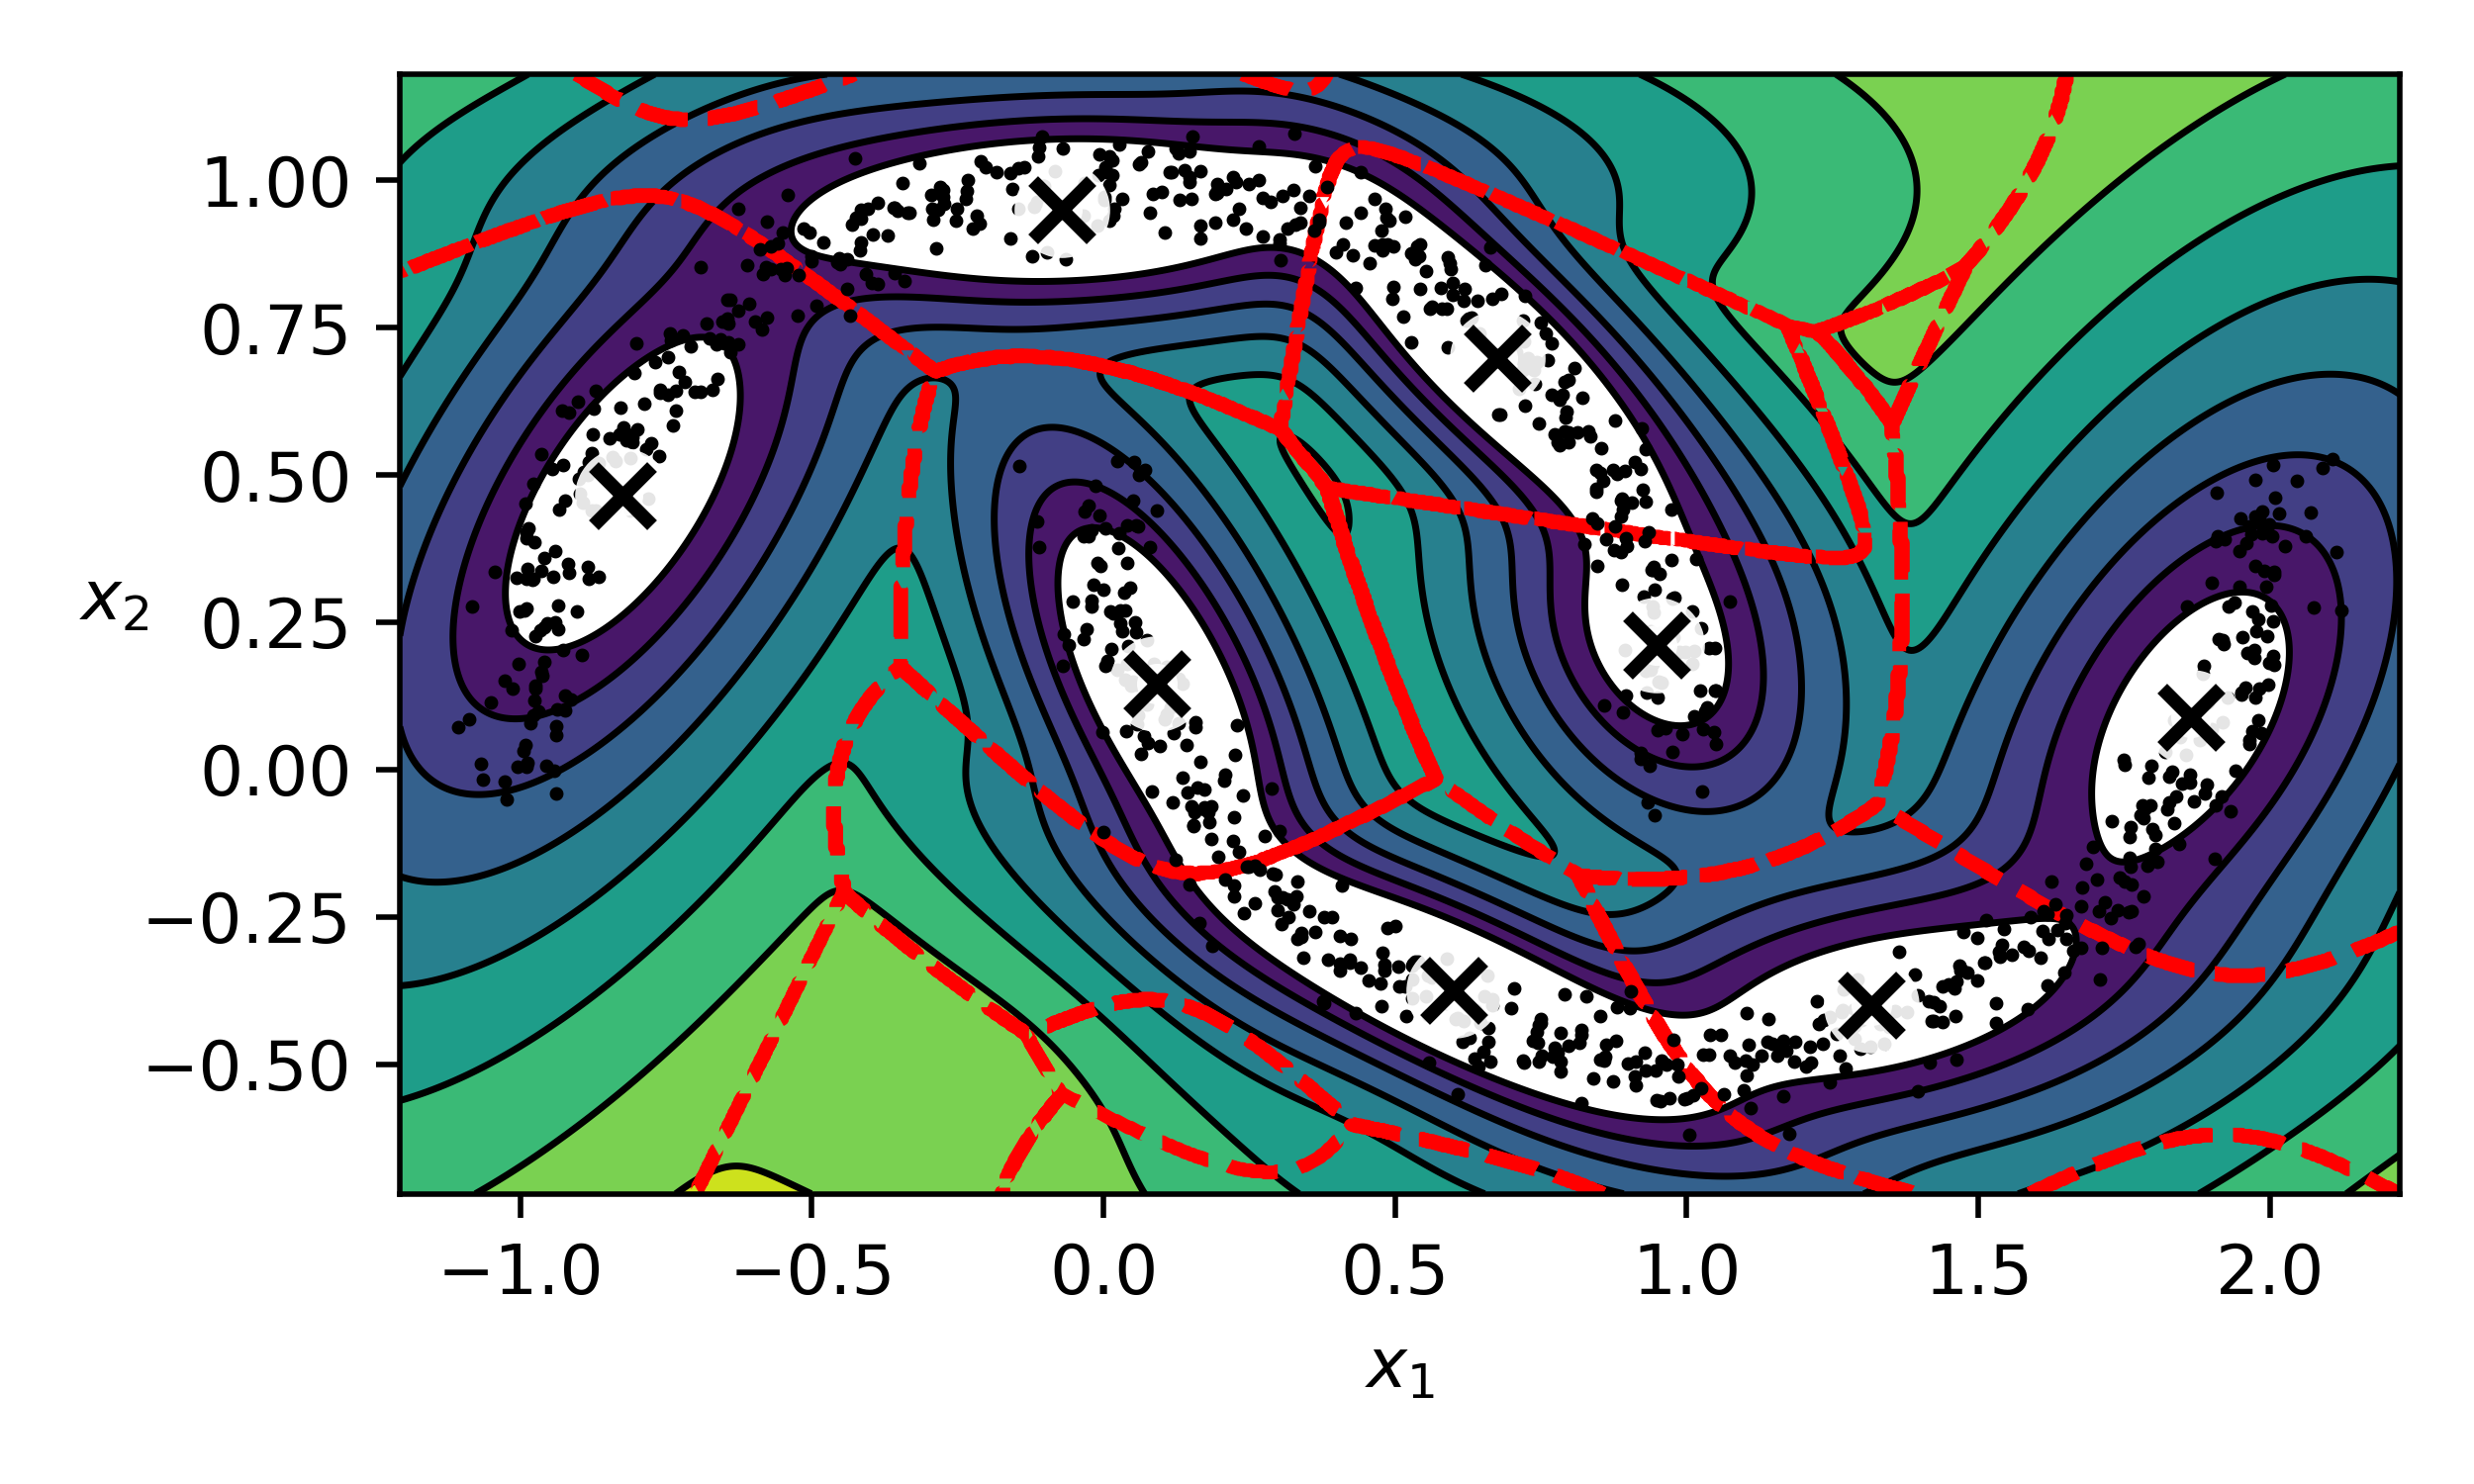
\includegraphics[width=7cm, height=7cm, keepaspectratio]{images/generative_26.png}
\end{center}
\end{column}
\end{columns}
\end{frame}

\begin{frame}{Optimális generátorszám megtalálása}
\begin{columns}
\begin{column}{.5\textwidth}
A keverék modellek esetén \textbf{nem megbízható a könyök módszer és a sziluett sem}, mert ezek izotróp (azonos formájú) klaszterekkel képesek jól működni.\par\medskip
Ehelyett rendelkezésre áll a \textbf{BIC és AIC információs kritériumok}, amelyek a modell komplexitását és jóságát veszik alapul.
\end{column}
\begin{column}{.5\textwidth}
\only<1>{\begin{block}{BIC}
\[
BIC = log\left( m \right) - 2 \cdot log\left( \hat{L} \right)
\]
Ahol:
\begin{itemize}
	\item $m$: Az egyedek száma
	\item $p$: A modell paramétereinek száma
	\item $\hat{L}$: A modell likelihood függvényének maximuma
\end{itemize}
\end{block}}
\only<2>{\begin{block}{AIC}
\[
AIC = 2 \cdot p - 2 \cdot log\left( \hat{L} \right)
\]
Ahol:
\begin{itemize}
	\item $m$: Az egyedek száma
	\item $p$: A modell paramétereinek száma
	\item $\hat{L}$: A modell likelihood függvényének maximuma
\end{itemize}
\end{block}}
\end{column}
\end{columns}
\end{frame}

\begin{frame}{Valószínűség és likelihood}
\begin{columns}
\begin{column}{.5\textwidth}
\begin{block}{Valószínűség}
A valószínűség azt adja meg, mekkora esélye van egy $x$ kimenetelnek, ha adott $\theta$ paraméterhalmaz.
\end{block}
\begin{block}{Likelihood}
A likelihood azt jelenti, hogy mennyire valószínű egy $\theta$ paraméterhalmaz, miután ismert $x$ kimenetel. 
\end{block}
\end{column}
\begin{column}{.5\textwidth}
\begin{center}
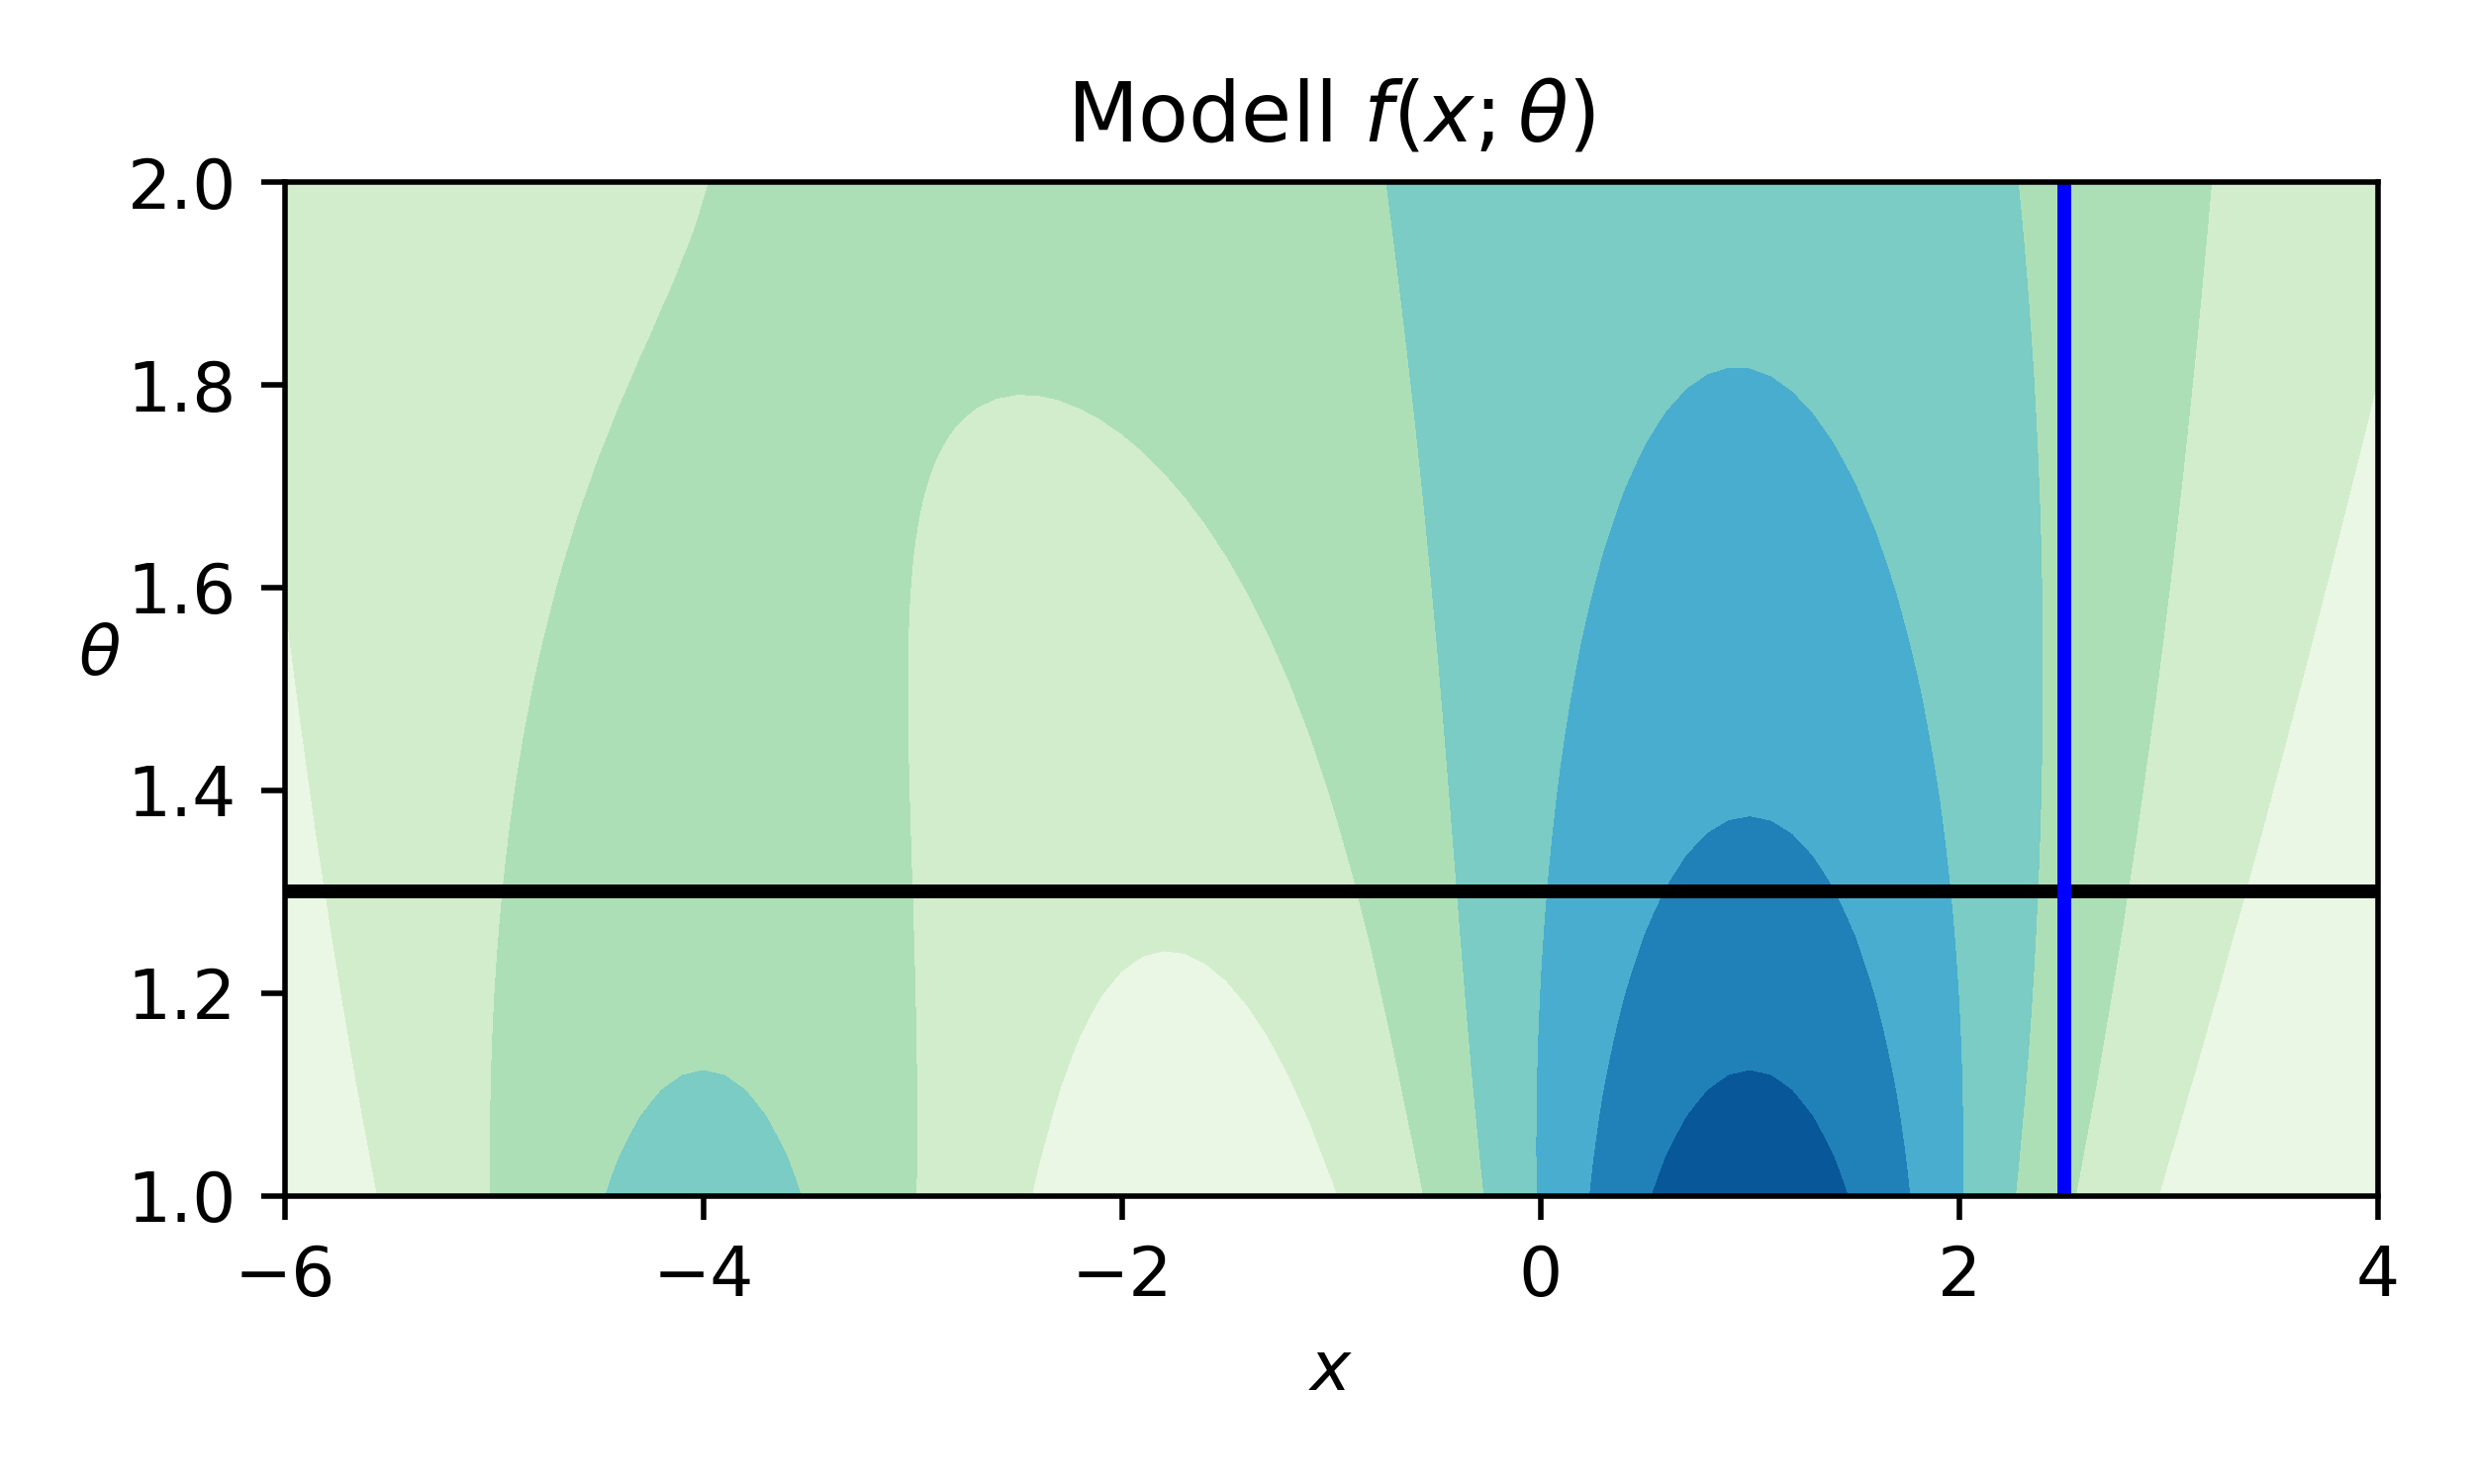
\includegraphics[width=6cm, height=7cm, keepaspectratio]{images/generative_28.png}
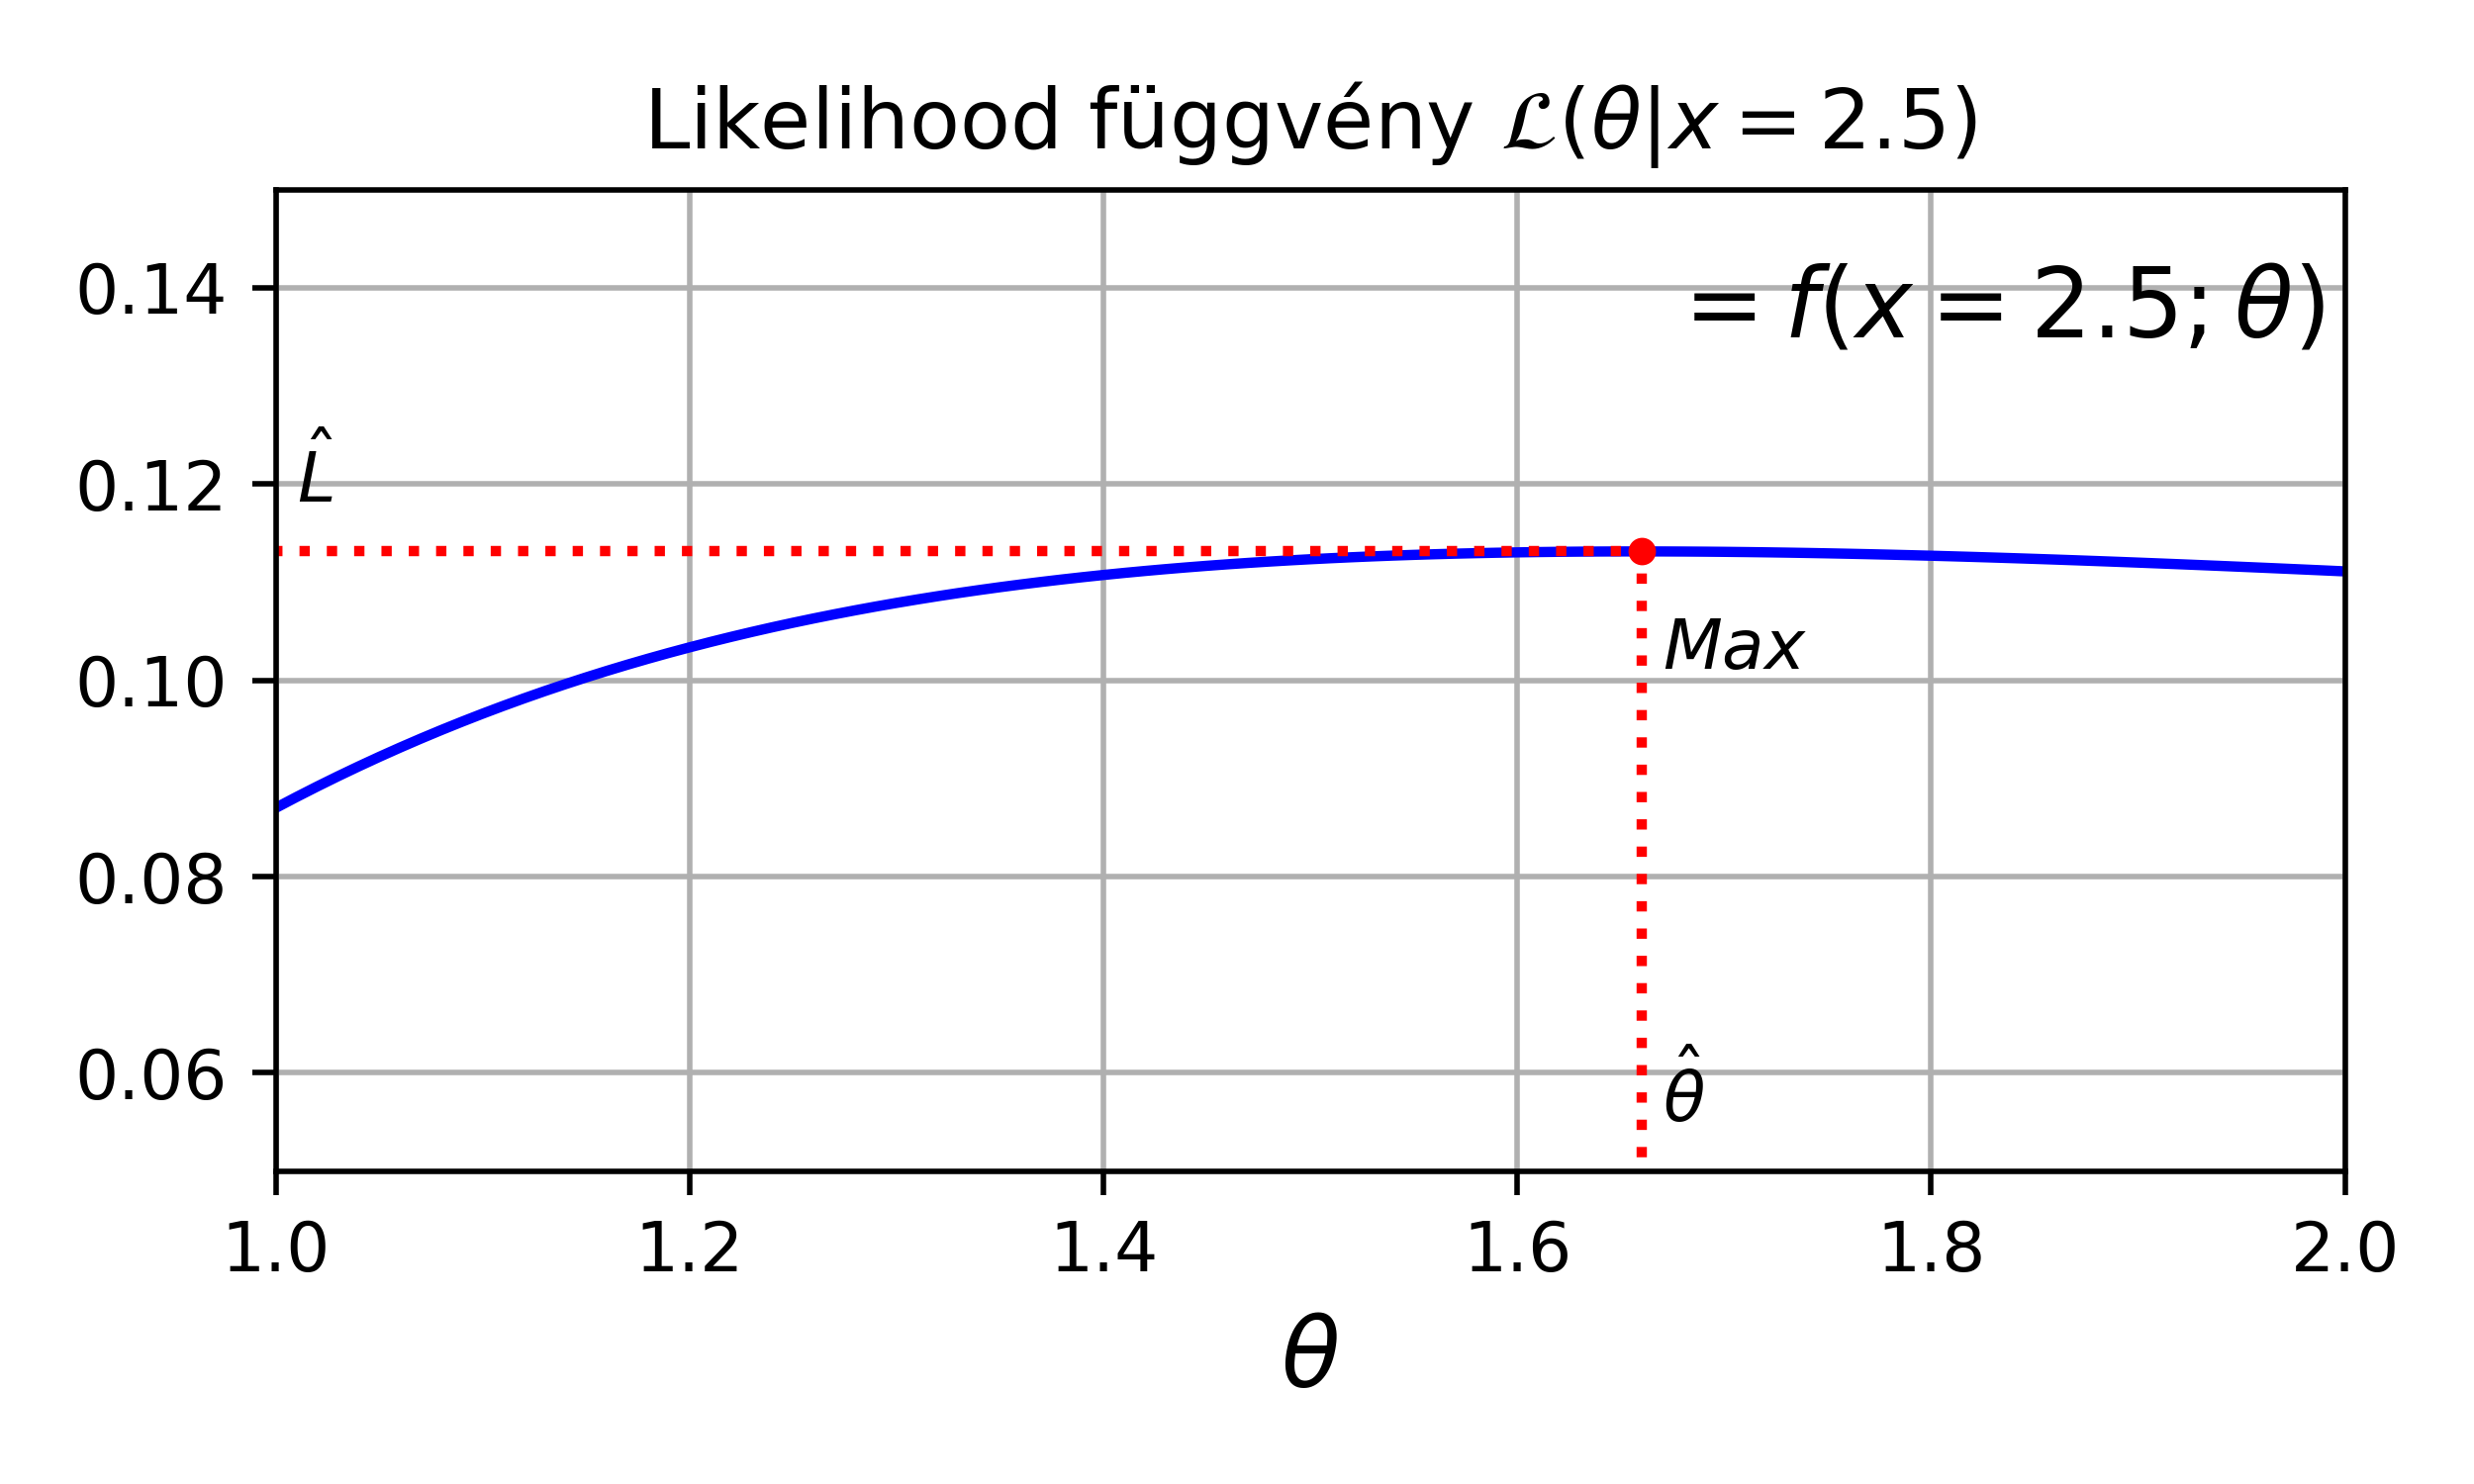
\includegraphics[width=6cm, height=7cm, keepaspectratio]{images/generative_29.png}
\end{center}
\end{column}
\end{columns}
\end{frame}

\begin{frame}{BIC, AIC diagram}
Az optimális generátorszám ott található, ahol a minden $k$ generátorszámra kiszámolt BIC és AIC információs kritériumoknak a legalacsonyabb az értéke:\par\smallskip
\begin{center}
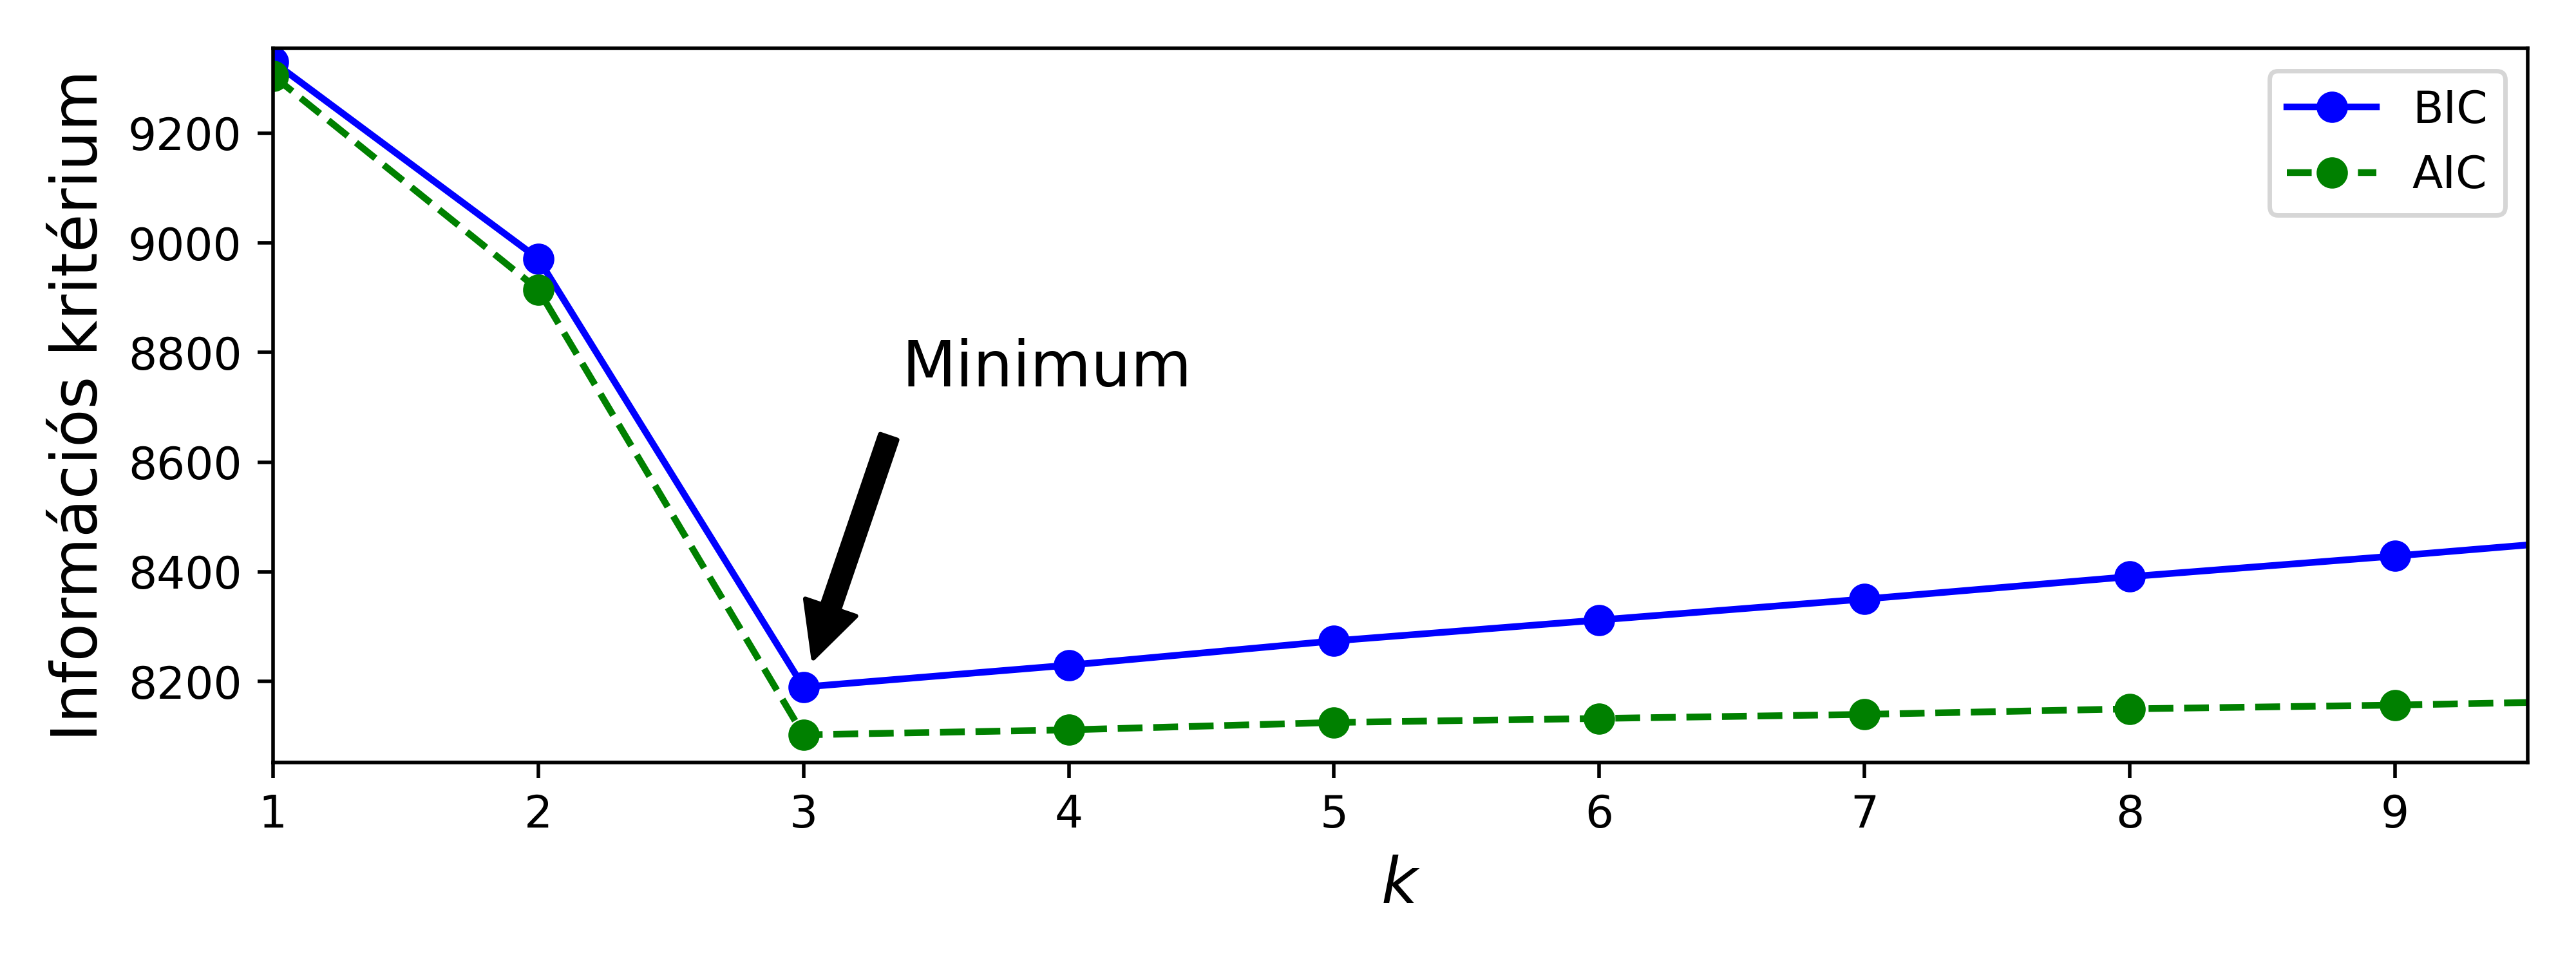
\includegraphics[width=12cm, height=7cm, keepaspectratio]{images/generative_32.png}
\end{center}
\end{frame}

\end{document}


























